\documentclass[aspectratio=169]{beamer}


\makeatletter
\newlength\beamerleftmargin
\setlength\beamerleftmargin{\Gm@lmargin}
\makeatother

%%%%%%% STYLE %%%%%%%%%%%%%%%%%%%%%%%%%%%%%%%%%%%%%%%%%%%%
% FONTS
\usepackage[proportional]{sourcesanspro}
\usepackage[T1]{fontenc}

\usepackage{soul}   % Rayer

% Rayer a un certain moment seulement
\newcommand<>{\sta}[1]{
  \alt#2{\st{#1}}{{#1}}
}


\usepackage{hyperref}
\usepackage{multirow}

% TITLE
\setbeamerfont{frametitle}{size=\large}


% MARGINS
\newenvironment{changemargin}[2]{%
  \begin{list}{}{%
    \setlength{\topsep}{0pt}%
    \setlength{\leftmargin}{#1}%
    \setlength{\rightmargin}{#2}%
    \setlength{\listparindent}{\parindent}%
    \setlength{\itemindent}{\parindent}%
    \setlength{\parsep}{\parskip}%
  }%
  \item[]}{\end{list}} 

% FOOTNOTES
\renewcommand{\thefootnote}{}
\renewcommand{\footnoterule}{}

% MATHS
\usepackage{amsmath, amssymb, amsfonts}
%\usepackage[OMLmathrm,OMLmathbf]{isomath}

% LISTS
%\usepackage{enumitem}

% Enumerate style
\setbeamertemplate{enumerate items}[circle]
\setbeamercolor{item projected}{bg=maincol,fg=bgcol}

\setbeamertemplate{itemize subitem}{\color{maincol}$\blacktriangleright$}
\setbeamertemplate{itemize item}{\color{maincol}$\blacktriangleright$}

% Description
\setbeamercolor{description item}{ fg=maincol}

% COLORS
\usepackage{xcolor}
%\input{~/Dropbox/Presentations/Templates/tangocolors.sty}

\definecolor{bgcol}{rgb}{1,1,1} % Background color
\definecolor{fgcol}{rgb}{0,0,0} % Foreground color

\definecolor{maincol}{RGB}{0, 107, 137} % Bleu canard %006b8b
\definecolor{col1}{RGB}{125, 72, 150} % Purple %7d4896
\definecolor{col2}{RGB}{178, 208, 76} % Light green %b0d04c
\definecolor{col3}{RGB}{123, 191, 210} % Blue
\definecolor{col4}{HTML}{2C5AA0} % Opposite of light green
\definecolor{col12A}{RGB}{169, 152, 100}
\definecolor{col12B}{RGB}{42, 117, 125}

%\definecolor{maincol}{HTML}{7D1935} % Rubis
%\definecolor{col1}{HTML}{4A96AD} % Blue
%\definecolor{col2}{HTML}{575042} % Brown

\definecolor{cl1}{HTML}{234BCD}
\definecolor{cl2}{HTML}{5D5B8F}
\definecolor{cl3}{HTML}{976C52}
\definecolor{cl4}{HTML}{D17D15}

\definecolor{mgray}{gray}{0.55}
\definecolor{dgray}{gray}{0.3}
\definecolor{lgray}{gray}{0.75}
\definecolor{gray70}{gray}{0.70}

% COLORS AND THEMES
\usecolortheme[named=maincol]{structure} 
\setbeamercolor{alerted text}{fg=maincol} 
\setbeamercolor{frametitle}{fg=maincol}
\setbeamercolor{structure}{fg=fgcol, bg=bgcol}



% TITLE SECTION
\newcommand{\titlesec}[3]{\begin{center}
  \vspace{1.5cm}
                           \parbox{0.8\textwidth}{\textcolor{#3}{\begin{center} \Large #1 \\ \vspace{0.75cm} {\small \textcolor{mgray}{#2}} \end{center}}} \end{center}
			  }

% DESSINS
%\usepackage{pgf}
\usepackage{tikz}

\usetikzlibrary{patterns}
\usetikzlibrary{positioning,shadows,backgrounds,decorations.pathreplacing}
\usetikzlibrary{fit, calc}
\usetikzlibrary{shapes, shapes.callouts, decorations.text}
\usetikzlibrary{arrows}
%\usepackage{pgfplots}
\usepackage{rotating}

% GENERAL LAYOUT
\setbeamertemplate{navigation symbols}{} 
\setbeamertemplate{blocks}[rounded][shadow=false]

\setbeamercolor*{author in head/foot}{parent=palette quaternary}
\setbeamercolor*{title in head/foot}{parent=palette quaternary}
\setbeamercolor*{date in head/foot}{parent=palette quaternary}
\setbeamercolor*{section in head/foot}{fg=mgray}
\setbeamercolor*{subsection in head/foot}{parent=palette quaternary}

\def \hbarfoot {2.5ex}
\def \dbarfoot {1.75ex}
\defbeamertemplate*{footline}{infolines theme}
{
  \leavevmode%
  \hbox{%
  %
  \begin{beamercolorbox}[wd=.33\paperwidth, ht=\hbarfoot, dp=\dbarfoot, center]{section in head/foot}%
    \usebeamerfont{author in head/foot}
    \insertshortauthor % Uncomment to add author's name in the foot
      \end{beamercolorbox}
      %
  \begin{beamercolorbox}[wd=.33\paperwidth, ht=\hbarfoot, dp=\dbarfoot, center]{section in head/foot}%
    \usebeamerfont{title in head/foot}
% ESEB, August 2017
  \end{beamercolorbox}%
  %
  \begin{beamercolorbox}[wd=.33\paperwidth, ht=\hbarfoot, dp=\dbarfoot, right]{bg=bgcol, fg=fgcol}%
    \usebeamerfont{date in head/foot}
    \insertframenumber{} %/ \inserttotalframenumber %
	\hspace*{2ex} 
  \end{beamercolorbox}}%
  \vskip0pt%
}


\addtobeamertemplate{footline}{%
  %\leavevmode%
  \color{maincol!50!white}% to color the progressbar
%  \hspace*{-\beamer@leftmargin}%
%  \rule{\beamer@leftmargin}{2pt}%
  \rule{\dimexpr \insertframenumber\paperwidth/\inserttotalframenumber}{\dimexpr -1.25pt+\dbarfoot}
  % next 'empty' line is mandatory!

%  \vspace{0\baselineskip}
\vspace{\dimexpr -\hbarfoot-\dbarfoot}
  {}
}


% BLOCKS

%\addtobeamertemplate{block begin}{\pgfsetfillopacity{0.}}{\pgfsetfillopacity{1}}
%\addtobeamertemplate{block beamercolorbox begin}{\pgfsetfillopacity{0.65}}{\pgfsetfillopacity{1}}
%\setbeamercolor{block title}{fg=maincol, bg=red}%use=structure,fg=black,
%     bg=white!10}
\setbeamercolor{block title}{bg=white!10, fg=maincol}
%\setbeamercolor{block body}{%use=structure,fg=black,
%     bg=white!10}
\setbeamerfont{block title}{size=\normalsize}



\newcommand{\smallblock}[3]{
\begin{minipage}[c]{#1}
  \begin{block}{#2}
   #3
  \end{block}
\end{minipage}
}





% ROTATE TEXT FOR CREDITS
\usepackage{graphics}
\definecolor{lgray}{gray}{0.75}
\newcommand{\piccredit}[1]{\hspace{0.1em}\rotatebox{90}{\tiny \textcolor{gray70}{(c) #1}}}
\newcommand{\picc}[1]{ \rotatebox{90}{\tiny \textcolor{lgray}{#1}}}

% STROKE
%\usepackage{ulem}

% TABLES
\usepackage{array}

% ANIMATIONS - MOVIES
\usepackage{multimedia}


\newcommand{\refpaper}[3]{
\begin{flushright}
\textcolor{gray50}{\tiny #1 (#2), \textit{#3}}
\end{flushright}
}

%% Maths

%\newcommand{\mat}[1]{\mathrm{\mathbf{#1}}}
\newcommand{\mat}[1]{\mathbf{#1}}
\DeclareMathOperator{\Tr}{Tr}
\newcommand{\Trace}[1]{\Tr \left( #1 \right)}

%% Command for Raising pictures
\newcommand{\raisepic}[1]{\raisebox{-\height}{#1}}
\newcommand{\midpic}[2]{\raisebox{-#2\height}{#1}}

% Checkmarks
\usepackage{pifont}
\newcommand{\cmark}{\ding{51}}%
\newcommand{\xmark}{\ding{55}}%



% REFERENCES
%% References
\newcommand{\pprref}[2]{\textcolor{mgray}{#1 (#2)}}
%\usepackage{natbib}
% Remove the icon before each item
\setbeamertemplate{bibliography item}{}

% Only number References slides if they are more than 1
\setbeamertemplate{frametitle continuation}[from second]

%remove line breaks
\setbeamertemplate{bibliography entry title}{}
\setbeamertemplate{bibliography entry location}{}
\setbeamertemplate{bibliography entry note}{}

%\setbeamercolor*{bibliography entry title}{fg=fgcol}
\setbeamercolor*{bibliography entry author}{fg=maincol}
%\setbeamercolor*{bibliography entry note}{fg=fgcol}
%\setbeamercolor*{bibliography entry location}{fg=fgcol}


% In text?
\newcommand{\refstyle}[1]{\scriptsize  \textcolor{dgray}{#1}}

% As footnote
\newcommand{\theref}[1]{{\footnotetext{\begin{flushright} \refstyle{#1} \end{flushright} } }}

% NOTES
%\setbeamertemplate{note page}[plain]
\setbeamerfont{note page}{size=\scriptsize}

% APPENDIX
% Change numbering for the appendix
\newcommand{\backupbegin}{
   \newcounter{framenumberappendix}
   \setcounter{framenumberappendix}{\value{framenumber}}
}
\newcommand{\backupend}{
   \addtocounter{framenumberappendix}{-\value{framenumber}}
   \addtocounter{framenumber}{\value{framenumberappendix}} 
}

% HYPERLINKS
\setbeamercolor{button}{bg=maincol,fg=bgcol}

% DESCRIPTIONS
\defbeamertemplate{description item}{align left}{\insertdescriptionitem\hfill}


\newcommand{\btVFill}{\vskip0pt plus 1filll}
\newcommand{\EE}{\mathbb{E}}
\newcommand{\PP}{\mathbb{P}}

%%%%%%%%%%%%%%%%%%%%%%%%%%%%%%%%%%%%%%%%%%%%%%%%%%%%%%

%\colorlet{colA}{ta2chameleon}
%\colorlet{colB}{ta2chocolate}

% Colors for the legends
\definecolor{pinka}{HTML}{DA8DAC}
\definecolor{pinkb}{HTML}{ac0045}
\definecolor{pinkc}{HTML}{4c001e}
\definecolor{pinkd}{HTML}{ecc6d5}


%\newcommand{\sderivv}[3]{\left.\frac{\partial #1}{\partial #2}\right|_{#3 =0}}
\newcommand{\sderivv}[3]{\left. \frac{\partial #1}{\partial #2} \right|_{\delta =0}}

\newcommand{\ssum}[2]{{\textstyle \sum\limits_{#1}^{#2}}}

\newcommand{\bb}{\mathsf{b}}
\newcommand{\cc}{\mathsf{c}}
\newcommand{\dd}{\mathsf{d}}

\newcommand{\demesize}{n}
\newcommand{\nbdemes}{N_d}
\newcommand{\Qin}{Q_{\textsf{in}}}
\newcommand{\Qout}{Q_{\textsf{out}}}
\newcommand{\selstr}{\delta}

% Environment for slides without headline
\makeatletter
    \newenvironment{withoutheadline}{
        \setbeamertemplate{headline}[default]
        \def\beamer@entrycode{\vspace*{-\headheight}}
    }{}
\makeatother

% To point at term in equation
\newcommand\tikzmark[1]{%
\tikz[remember picture, overlay] \node[inner xsep = 0pt] (#1) {};
}

% References
\newcommand{\citeref}[1]{\footnotesize \textcolor{mgray}{#1}}

\begin{document}

% TITLE PAGE
\begin{withoutheadline}
\begin{frame}
\vspace{-\baselineskip}
\begin{center}

\begin{tikzpicture}
\node[opacity=0.3]{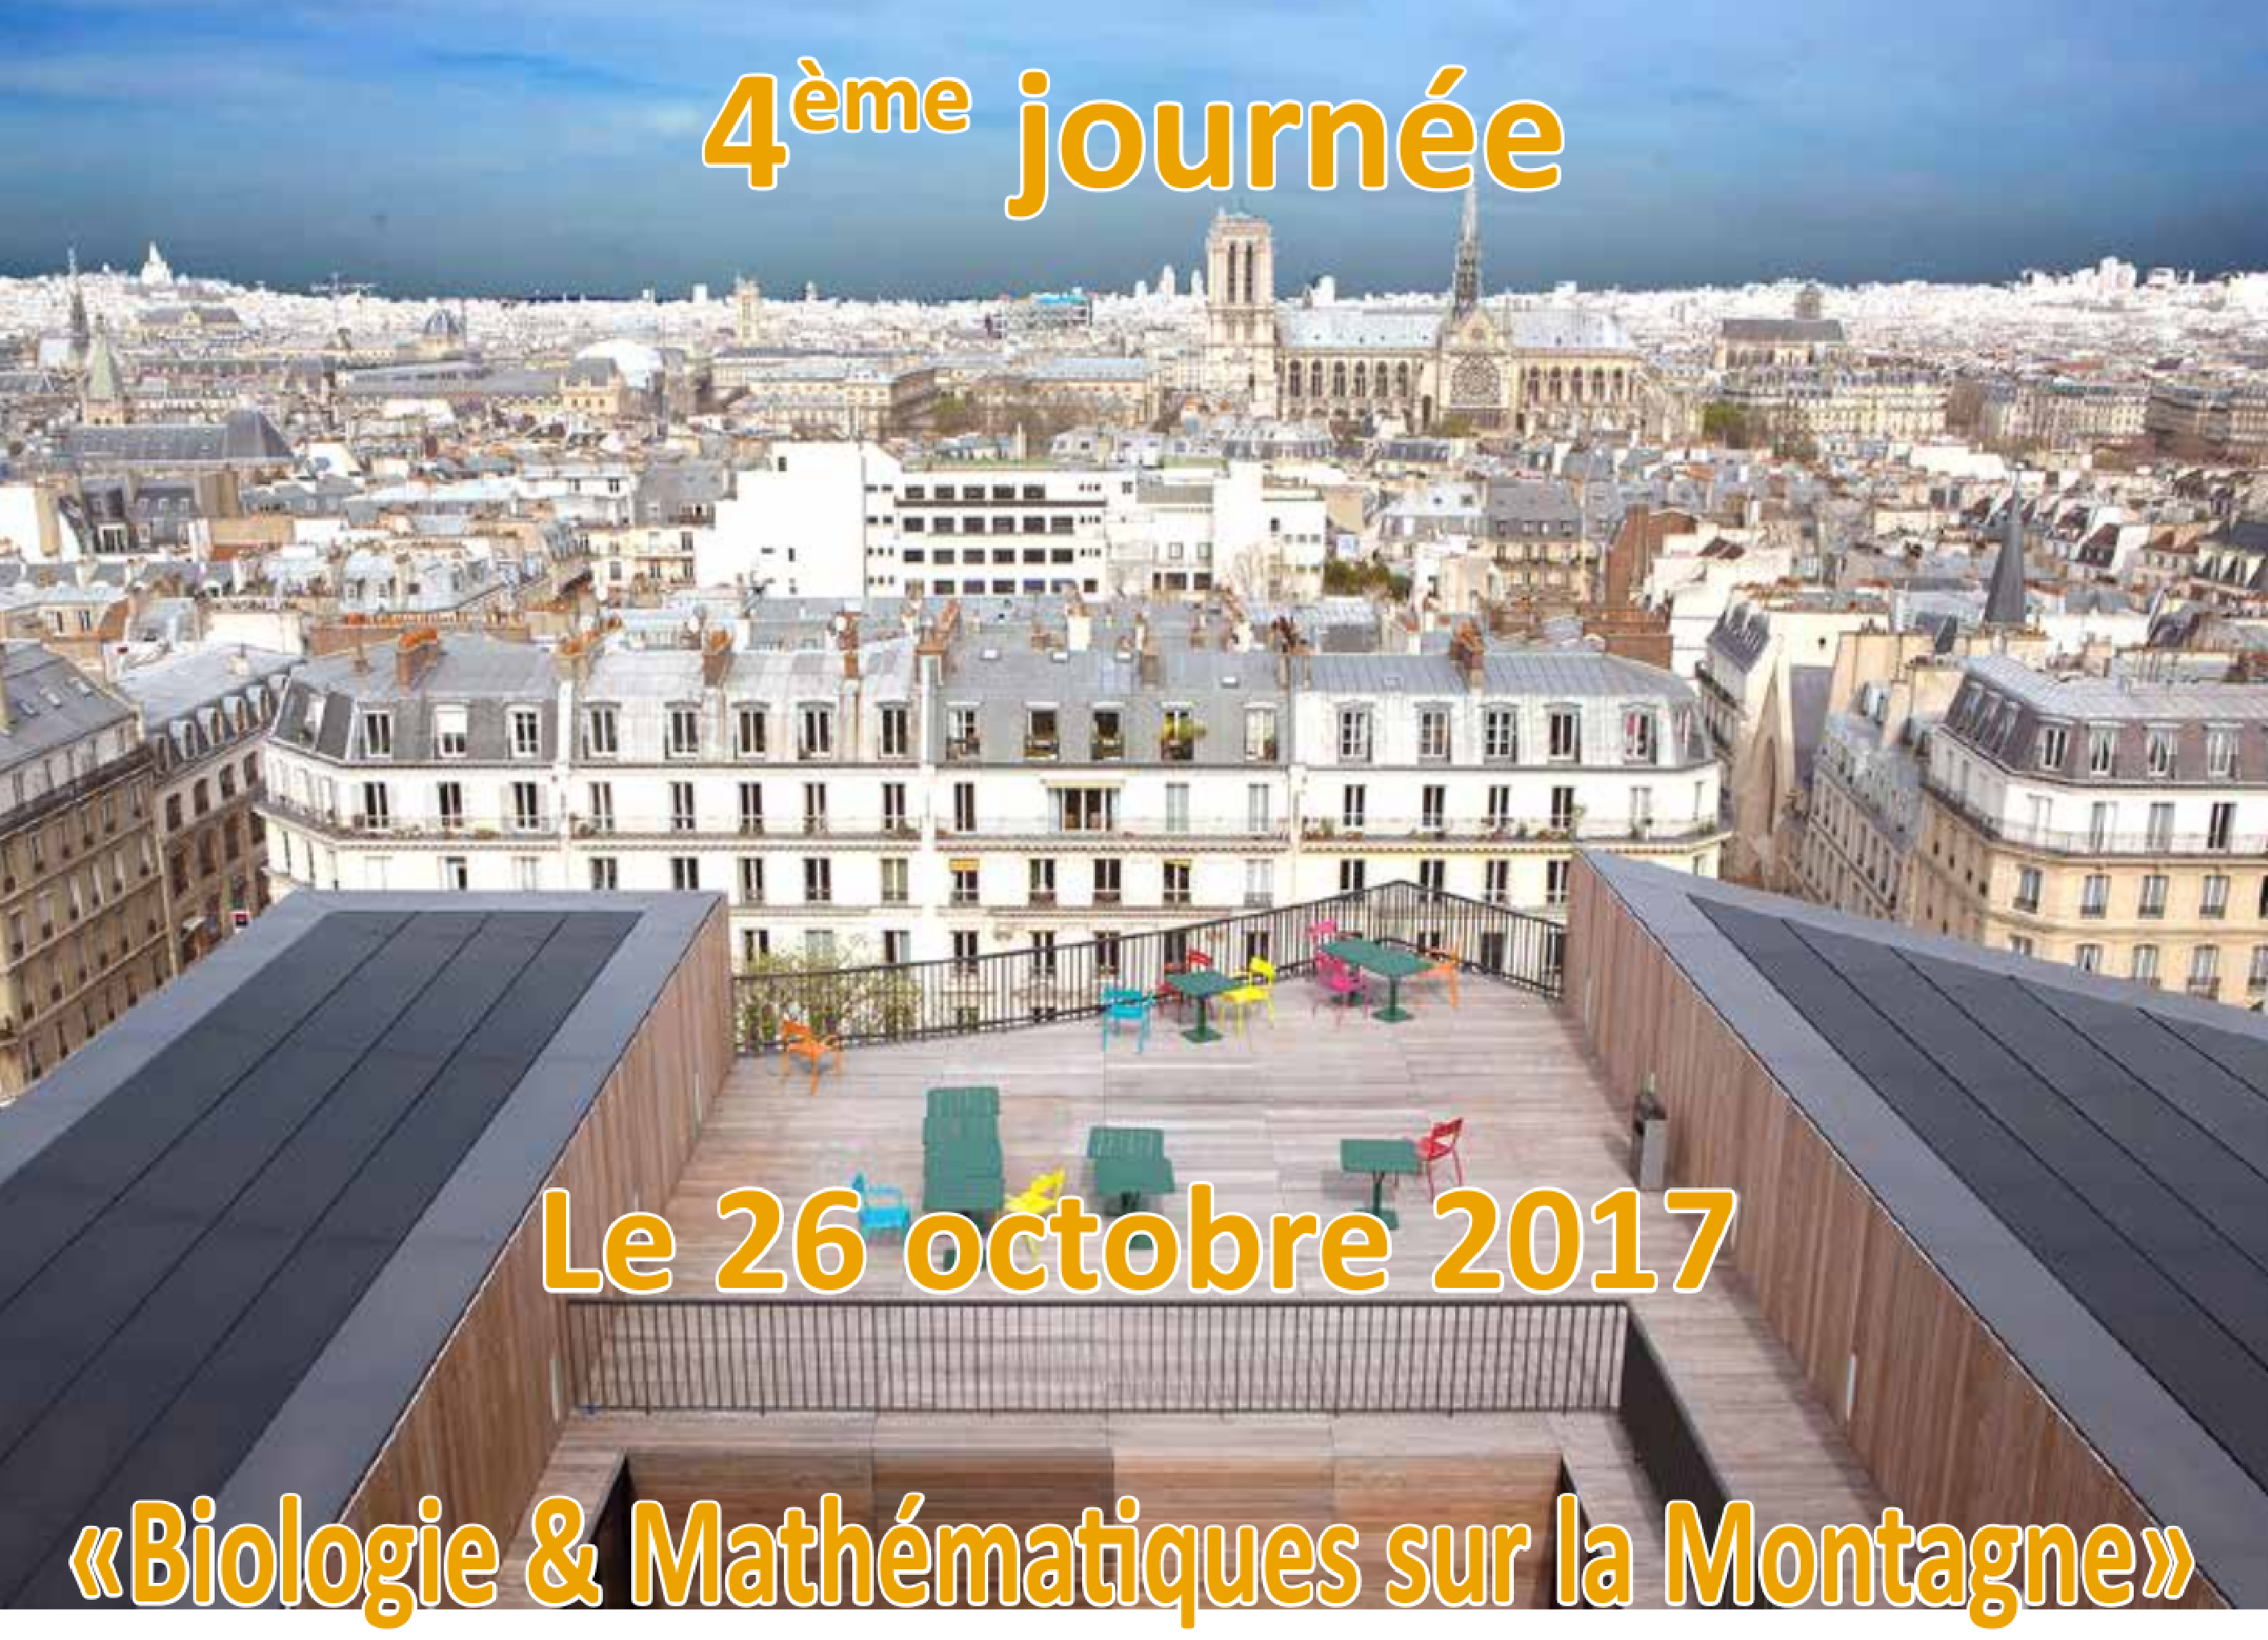
\includegraphics[height=\paperheight]{../Pics/afficheMBM.pdf}};

\node[text width=0.8\textwidth, font=\Large, align=center, color=maincol]at(0,1)(tit){ Social evolution in structured populations};
%Fidelity of parent-offspring transmission\\ and the evolution of social \mbox{behavior} in subdivided populations.};

\tikzstyle{nameauthor}=[inner sep=2pt, draw=none, anchor=base]
\def \dhn {2.25cm}
\node[below=2em of tit, nameauthor](FD){Florence D\'ebarre};

\node[below=-0.35cm of FD](sFD){}; % Removing pic because looks odd with single author
\tikzstyle{twee}=[font=\footnotesize, minimum height=2em]
\node[below=0cm of sFD, twee](tFD){@flodebarre};
\node[left=0cm of tFD]{\includegraphics[height=1em]{/home/florencedebarre/Dropbox/Presentations/GlobalPics/twitter.pdf}};

\node[below = 0.75cm of FD, align=center, font =\footnotesize]{ CNRS \\ Centre de Interdisciplinaire de Recherche en Biologie, Paris};
\end{tikzpicture}


%    \hspace*{-\beamerleftmargin}%

\end{center}
\end{frame}
\end{withoutheadline}

\section{Introduction}

\subsection{Puzzle of altruism}

\begin{withoutheadline}
\begin{frame}
\begin{center}
\begin{tikzpicture}

\node[opacity=1]{
\includegraphics[width=0.5\textwidth]{../Pics/puzzle.pdf}};
\def \hh {0.8cm}
\def \rad {2.5cm}
\tikzstyle{dck}=[inner sep=0pt, circle]
\tikzstyle{lnk}=[line width=1.5pt, draw=fgcol]

\uncover<2->{
%Cover puzzle
\node[minimum width = \textwidth, minimum height = \textheight, fill = white, fill opacity = 0.8]at(0,0){};

% Focal individual
\node[dck](cdc)at(-0.5*\rad,0){
\includegraphics[height=\hh]{../Pics/typeA.pdf}};

\uncover<2-3>{
\node[dck] (c6) at($(cdc)+(0:\rad)$){
\includegraphics[height=\hh]{../Pics/type0.pdf}};
}

\draw[lnk, ->] (cdc)--(c6){} node[midway, anchor = south]{
\includegraphics[height=0.75cm]{../Pics/gift.pdf}};

% Cost
\node[dck] at($(cdc)+(90:0.3*\rad)$){
\includegraphics[height=0.5cm]{../Pics/coins.pdf}};
}


% Add examples
\uncover<3>{
\tikzstyle{thepic}=[text width=2.5cm, align=center]

\node[thepic, anchor=east] at(-\rad, \rad){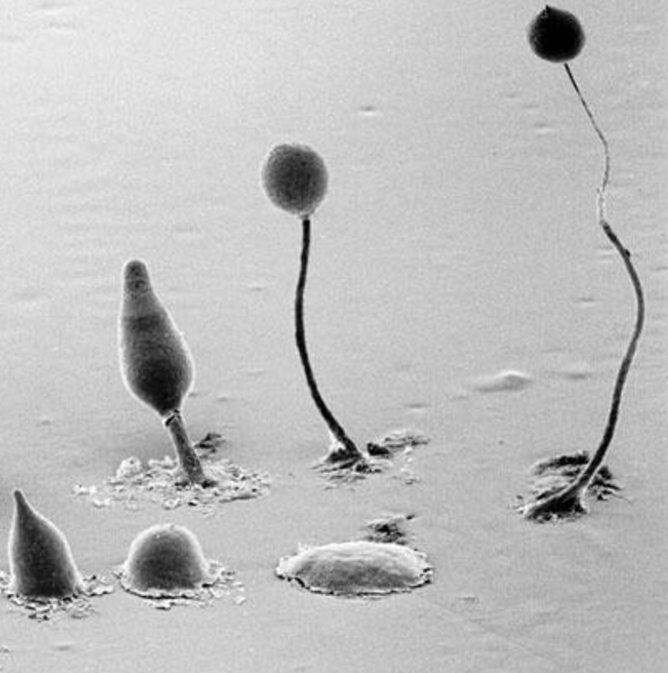
\includegraphics[width=0.9\columnwidth]{../Pics/socex_dictyostelium.pdf}\piccredit{Grimson \& Blanton}};

\node[thepic, anchor=west] at(\rad, \rad){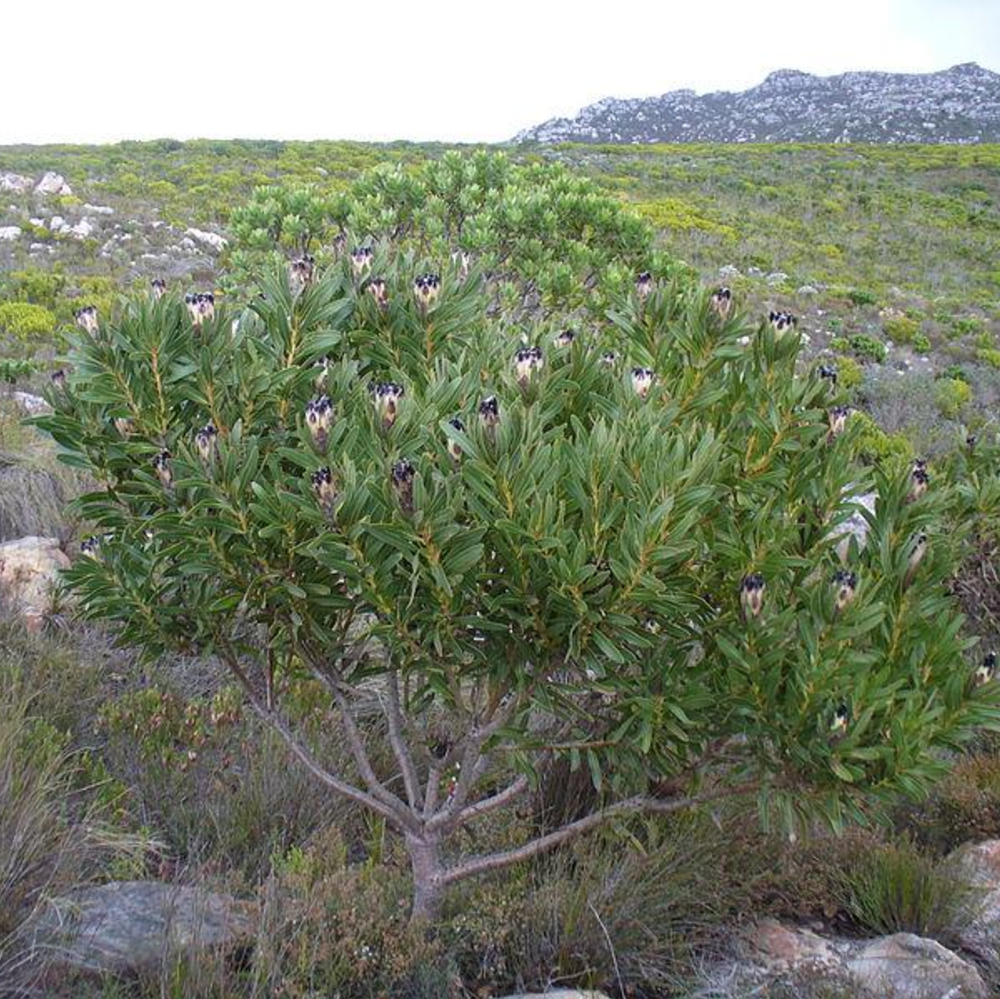
\includegraphics[width=0.9\columnwidth]{../Pics/socex_Protea_lepidocarpodendron.pdf}\piccredit{Wikimedia}
};

\node[thepic, anchor=east] at(-\rad, -\rad){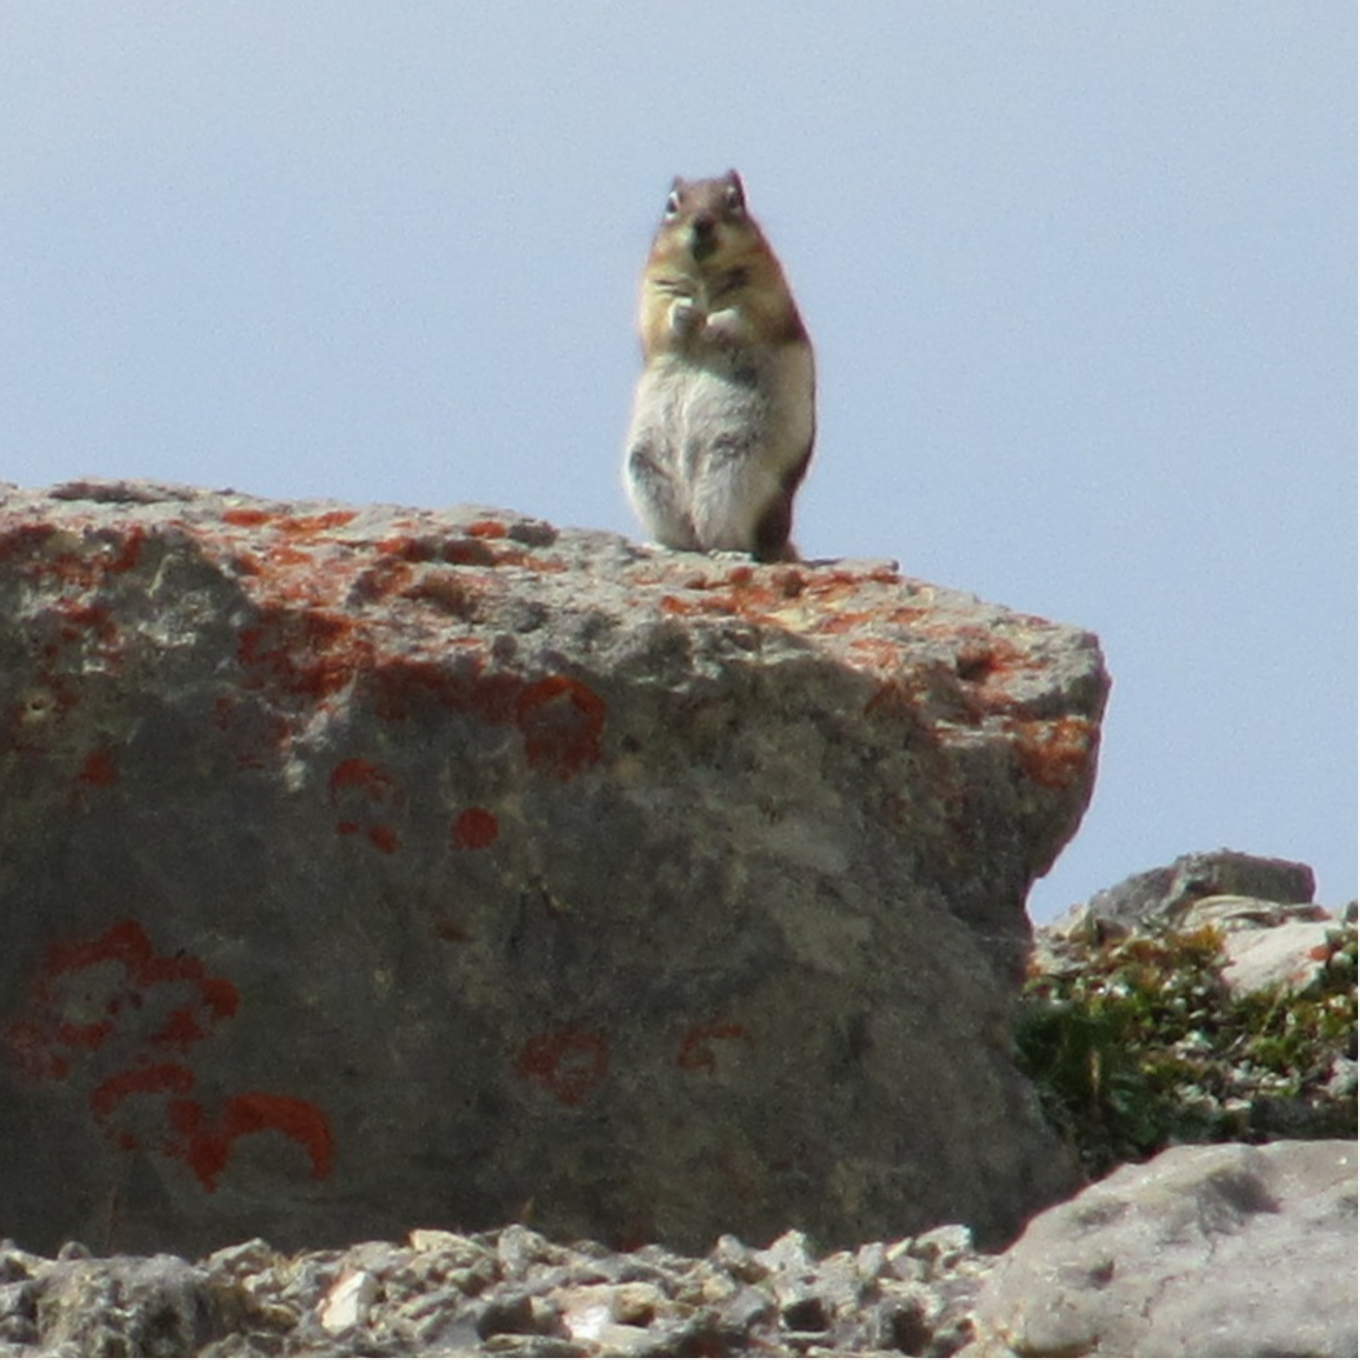
\includegraphics[width=0.9\columnwidth]{../Pics/socex_sentinelle.pdf}\piccredit{FD}
};

\node[thepic, anchor=west] at(\rad, -\rad){
\includegraphics[width=0.9\columnwidth]{../Pics/socex_superman.pdf}\piccredit{picturesforcoloring.com}
};
} % end examples uncover

\uncover<4>{
% Relatedness
\node[dck, circle, fill=none, draw=none] at (c6){
\includegraphics[height=\hh]{../Pics/typeA.pdf}};

\path[] (cdc)--(c6){} node[midway, anchor = north, yshift=-1cm, font=\large]{Assortment / Relatedness};

} % end uncover


\end{tikzpicture}
\end{center}
\end{frame}
\end{withoutheadline}

\subsection{Relatedness and spatial structure}

\begin{frame}{Spatial structure, population viscosity and altruism}
\begin{center}

\only<1>{
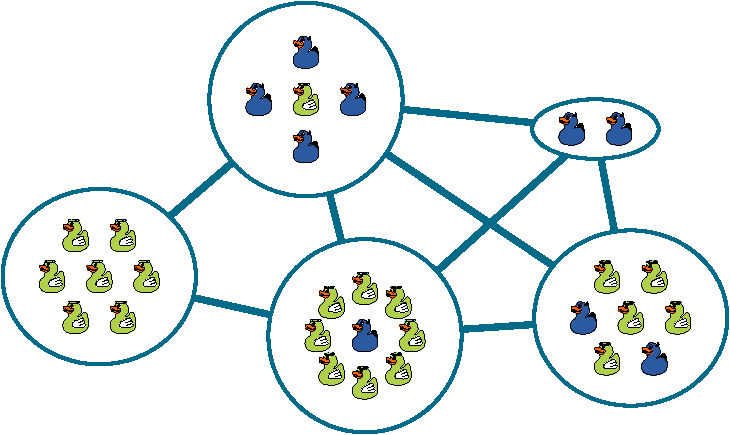
\includegraphics[width = 0.8\textwidth]{../TeXPics/subdivPopPic.pdf}
}

\uncover<2->{
\begin{tikzpicture}
\tikzstyle{popn}=[ellipse, draw=maincol, line width=1.5pt, inner sep = 0pt]
\tikzstyle{dck}=[inner sep=0pt, circle]
\def \rad {1.75cm}
\def \hpic {0.75cm}
\def \theduck {
\includegraphics[height=\hpic]{../Pics/empty.pdf}}

\def \TA {
\includegraphics[height=\hpic]{../Pics/typeA.pdf}}
\def \TB {
\includegraphics[height=\hpic]{../Pics/typeB.pdf}}

\node[dck]at(0,0) (d1){\TA};
\foreach \i in {1,...,6}{
\node[dck] (d1\i) at($(d1)+(\i*60:\rad)$){\TA};
}

\node[popn, fit=(d11)(d12)(d13)(d14)(d15)(d16)] (c1){};


\foreach \i in {1,...,6}{
\uncover<3->{
\node[]at(30+\i*60:0.5*\rad){
\includegraphics[height = 0.5cm]{../Pics/gift.pdf}};
}
\uncover<4->{
\node[rotate = \i*60+90]at(\i*60:0.5*\rad){
\includegraphics[height = 1cm]{../Pics/sword90.pdf}};
}
}

\only<5>{
\node[right = of c1, draw]{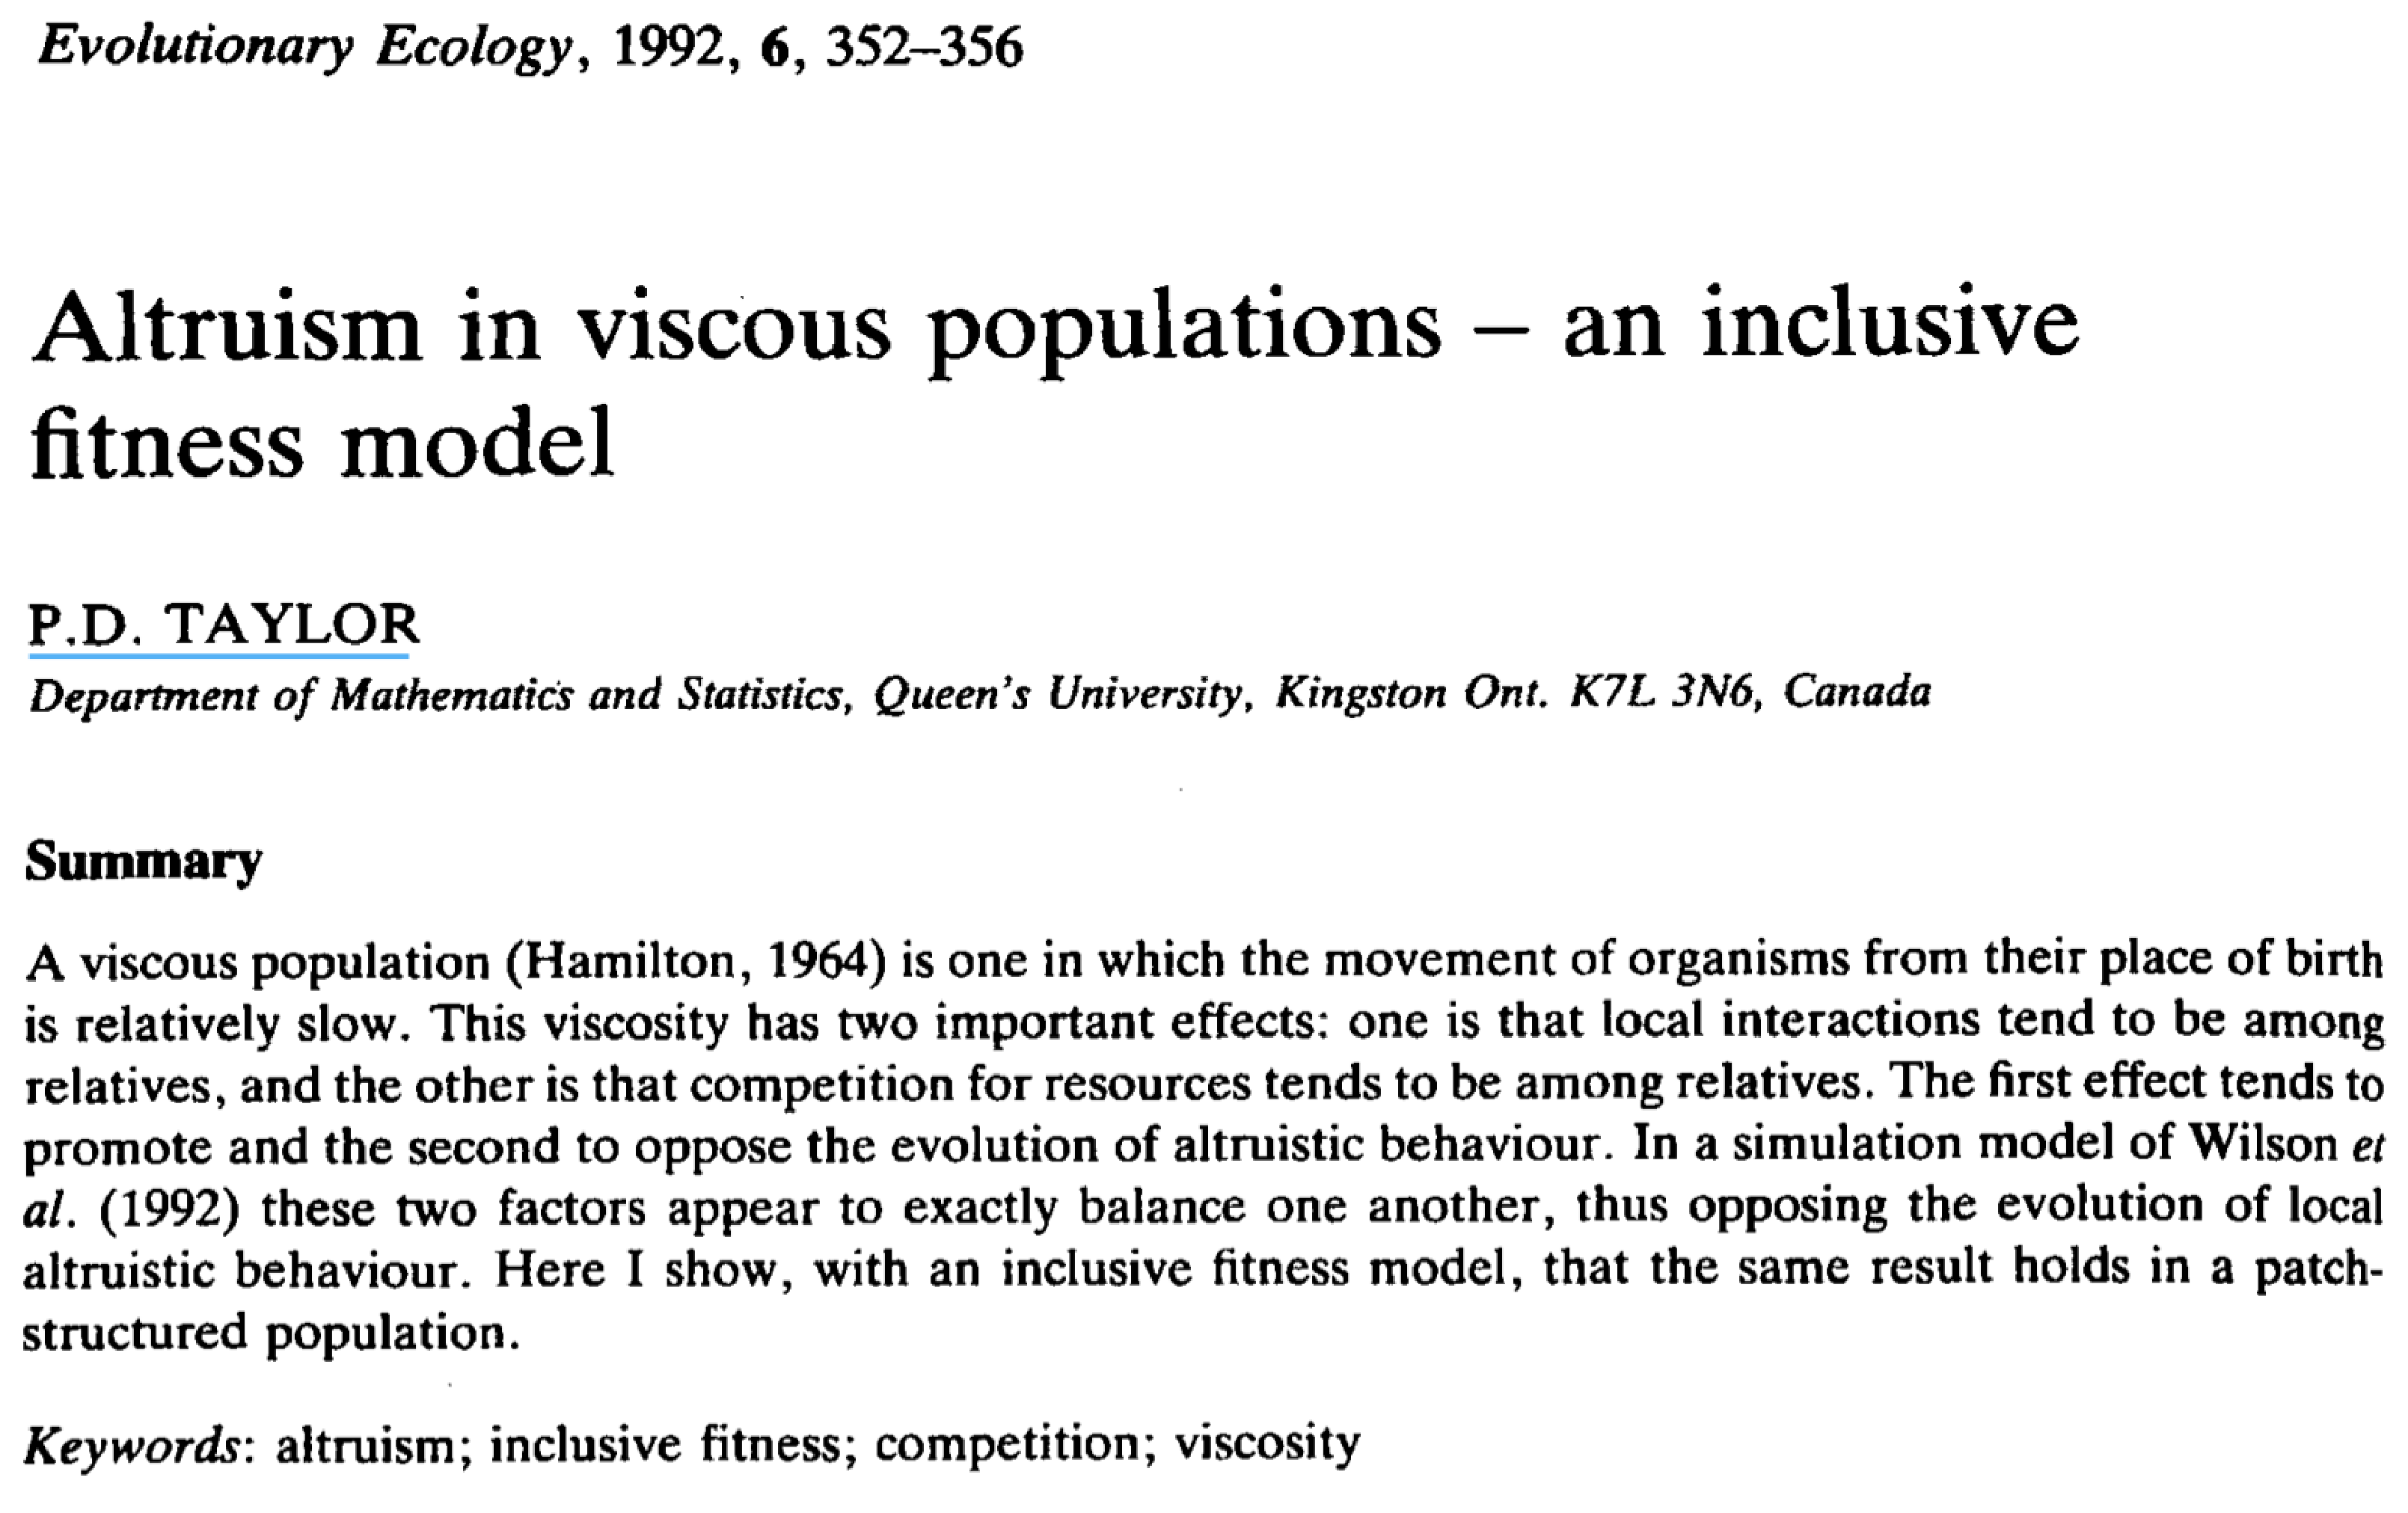
\includegraphics[width = 0.45\textwidth]{../Pics/Taylor1992.pdf}};
}
\end{tikzpicture}
}
\end{center}
\end{frame}

\subsection{Subdivided populations}

\begin{frame}{Subdivided population -- Island model}

$\nbdemes$ demes \uncover<2->{of $\demesize$ individuals each (total population size $N = \demesize \,\nbdemes$)}
\begin{center}

\begin{tikzpicture}
\tikzstyle{bigpop}=[circle, line width = 0.7pt, draw = none, fill = maincol!40, minimum width = 2.75cm]

\node[bigpop]at(0,0)(p4){};
\node[bigpop]at(2.5,2)(p3){};
\node[bigpop]at(2.5,-2)(p2){};
\node[bigpop]at(5,0)(p1){};
\node[bigpop]at(7.5,2)(p5){};
\node[bigpop]at(7.5,-2)(p6){};
\node[bigpop]at(10,0)(p7){};

\uncover<2->{
\def \wsmall {0.7cm}
\tikzstyle{site}=[circle, line width = 1.5pt, draw = maincol, fill=bgcol, minimum width = \wsmall]

\def \rad {0.85cm}
\foreach \i in {1,...,7}{
\foreach \j in {1,...,3}{
\node[site] at ($(p\i) + (90+\j * 120:\rad)$) (p\i\j){};
}
\node[site] at (p\i) (p\i4){};
}

% Philopatry
\uncover<3->{
\path (p1) edge [loop above, ->, looseness = 5, line width = 4pt, font = \large] node [above]{$1-m$} (p1);
}

% Dispersal
\uncover<4->{
\foreach \i in {2,...,7}{
\path[line width =1.5pt, ->, draw](p1)--(p\i);
}
\node[align = center, below = 0cm of p1, text width = 3cm, font = \large]{$m$\\Emigration probability};
}

\uncover<5->{
\tikzstyle{focusing}=[circle, minimum width = \wsmall, fill opacity = 0.8]
\node[focusing, fill = mgray] at (p14){};

\node[anchor = north , draw, align = center, font = {\bf\large}]at(10, -1.75){\color{mgray}focal \\ {\uncover<6->{\color{col1} in}} \\ {\uncover<7->{ \color{col2} out}}};

}

\uncover<6->{
\foreach \i in {1,...,3}{
\node[focusing, fill = col1] at (p1\i){};
}
}

\uncover<7->{
\foreach \i in {2,...,7}{
\foreach \j in {1,...,4}{
\node[focusing, fill = col2] at (p\i\j){};
}}
}



% Add ducks
\foreach \i in {1,...,7}{
\foreach \j in {1,...,4}{
\node[]at(p\i\j) {
\includegraphics[height = 0.6cm]{../Pics/type0.pdf}};
}}

% Add presents
\uncover<8->{
\foreach \i in {1,...,7}{
\foreach \j in {1,...,3}{
\node[]at($(p\i) + (30+ 120*\j:0.75cm)$){
\includegraphics[height = 0.5cm]{../Pics/gift.pdf}};
}}
}


}
\end{tikzpicture}
\end{center}

\end{frame}

\subsection{Previous results}

\begin{frame}{The choice of life-cycle matters}

\begin{center}
Constant population size ($N$), so
between two time steps, $\# 
\includegraphics[height=0.5cm]{../Pics/death} = \# 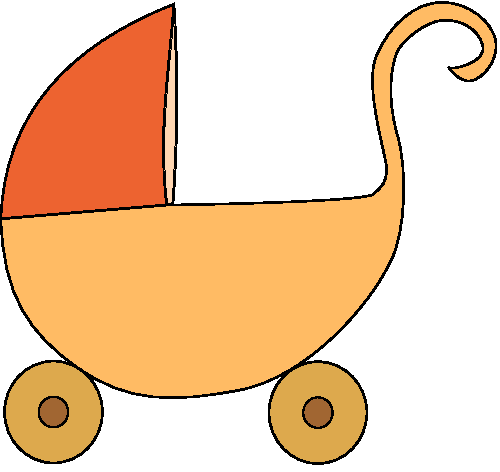
\includegraphics[height=0.5cm]{../Pics/birth}$.

\vspace{\baselineskip}

\uncover<2->{

\begin{tikzpicture}
\def \wpic {1cm}
\tikzstyle{lc}=[font=\large, minimum height = 1cm, draw=none, text depth = 0.2cm, color=maincol]
\def \dx {0.5cm}
\node[lc] (WF){Wright-Fisher};
\node[lc, right = \dx of WF] (BD){Moran Birth-Death};
\node[lc, right = \dx of BD] (DB){Moran Death-Birth};

\tikzstyle{tit2}=[lc, color = black]
\def \hh {2ex}
\def \dd {-0.5cm}
\node[tit2, below=\dd of WF](WFe){$N 
\includegraphics[height=\hh]{../Pics/death}$ \& $N 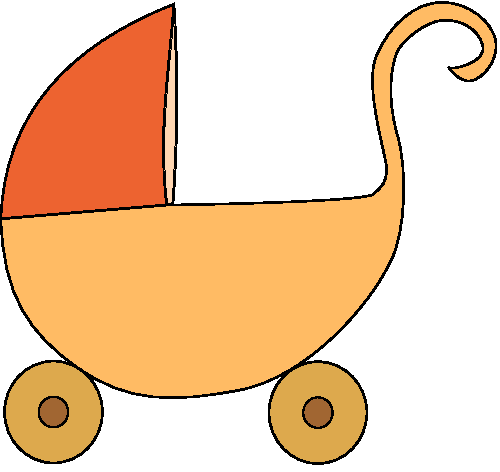
\includegraphics[height=\hh]{../Pics/birth}$};
\node[tit2, below=\dd of BD](BDe){$1 
\includegraphics[height=\hh]{../Pics/death}$ \& $1 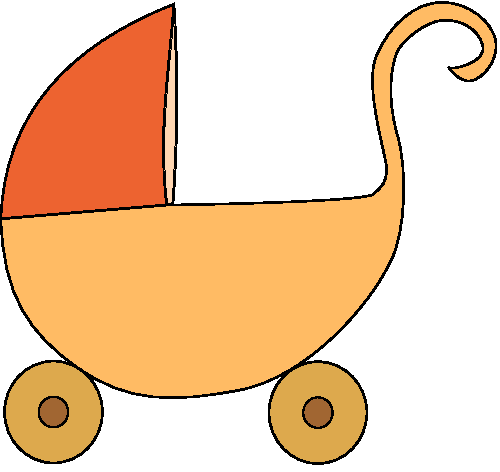
\includegraphics[height=\hh]{../Pics/birth}$};
\node[tit2, below=\dd of DB](DBe){$1 
\includegraphics[height=\hh]{../Pics/death}$ \& $1 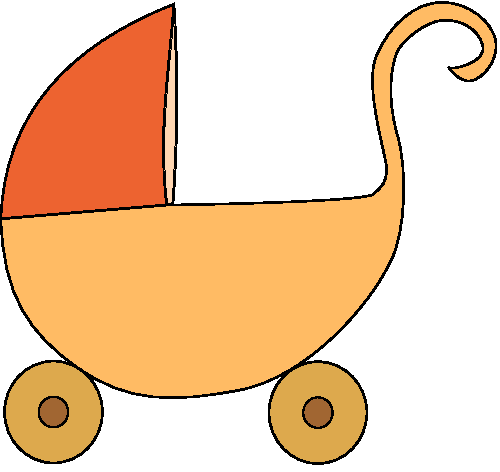
\includegraphics[height=\hh]{../Pics/birth}$};

\uncover<3->{
\tikzstyle{dck}=[]
\def \dy {0.4cm}
\node[dck, below = \dy of WF]{
\includegraphics[width =\wpic]{../Pics/typeB.pdf}};
\node[dck, below = \dy of BD]{
\includegraphics[width =\wpic]{../Pics/typeB.pdf}};
\node[dck, below = \dy of DB, font=\Huge]{
\includegraphics[width =\wpic]{../Pics/typeA.pdf} / 
\includegraphics[width =\wpic]{../Pics/typeB.pdf}};
}
\end{tikzpicture}
} %end uncover

\vspace{\baselineskip}
\uncover<3->{
In homogeneously structured populations, \\
with effects of social interactions on \textbf{fecundity}.
}
\end{center}

\footnote{\citeref{Ohtsuki et al. 2006; Taylor, Day \& Wild 2007; Taylor, Lillicrap, Cownden 2010}}

\end{frame}


\subsection{Transition mutation}

\begin{frame}{A common feature of models}
\begin{center}
\uncover<2->{
\begin{tikzpicture}
\def \TA {}
\def \TB {
\includegraphics[height = 1cm]{../Pics/typeB.pdf}}

\tikzstyle{dck}=[rectangle]
\def \parnt {1cm}
\def \offs {0.5cm}
\def \yb {-2cm}
\def \dpo {1.75}
\node[dck](a1) at(0,0){
\includegraphics[height = \parnt]{../Pics/typeA.pdf}};
\node[dck](d1) at(0,\yb){
\includegraphics[height = \parnt]{../Pics/typeB.pdf}};
\foreach \i in {1,...,5}{
\node[dck](ao\i)at(\dpo + 0.5*\i, 0){
\includegraphics[height = \offs]{../Pics/typeA.pdf}};
\node[dck](do\i)at(\dpo + 0.5*\i, \yb){
\includegraphics[height = \offs]{../Pics/typeB.pdf}};
}
\tikzstyle{arr}=[->, line width = 1.5pt, draw]
\path[arr] (a1)--(ao1);
\path[arr] (d1) -- (do1);

\uncover<3->{
\tikzstyle{cvr}=[inner sep = -3pt, rectangle, fill = bgcol]
\node[cvr, fit = (do2)]{};
\node[dck]at(do2){
\includegraphics[height = \offs]{../Pics/typeA.pdf}};
\node[cvr, fit = (ao4)]{};
\node[dck]at(ao4){
\includegraphics[height = \offs]{../Pics/typeB.pdf}};
}

\end{tikzpicture}
}

\uncover<4->{
\vspace{1em}
\begin{tikzpicture}
\node[text width = 0.6\textwidth, rounded corners, text opacity = 1, fill opacity = 0.5, fill = maincol, align = center, inner sep = 10pt]{What is the effect of population viscosity on the evolution of altruism when parent-offspring strategy transmission is \textbf{imperfect}?
};
\end{tikzpicture}
}

\end{center}
\end{frame}


\section{Model}

\subsection{Fidelity of transmission}

\subsubsection{What and why}

\begin{frame}{Fidelity of parent-offspring transmission}
\vspace{-1cm}
\begin{columns}[b]
\begin{column}{0.7\textwidth}
\begin{block}{Causes of imperfect strategy transmission}
\begin{itemize}
\item<1-> Mutation
\item<2-> Partial heritability
\item<3-> Cultural transmission (vertical)
\end{itemize}
\end{block}
\end{column}
\begin{column}{0.25\textwidth}
\uncover<1->{\includegraphics[width=\columnwidth]{/home/florencedebarre/Dropbox/Presentations/2016-07_ECMTB/Pics/kylo.pdf}}
\end{column}
\end{columns}

\uncover<4->{
\begin{block}{In the model}
\begin{center}
	\begin{tikzpicture}
	\def \xdist {2.75cm}
	\def \ydist {0.8cm}
	\def \dydist {0.5cm}
	\def \hh {0.65cm}
	\tikzstyle{circindiv}=[text width=0.65cm, inner sep=0pt, align=center] % Circle for individual type
	\tikzstyle{lin}=[line width=2pt, >=angle 45, draw=dgray] % Line type
	\tikzstyle{arr}=[->, lin] % Arrow type, using line type
	\tikzstyle{arrlab}=[inner sep=3pt, draw=none] % Label on arrow
	\tikzstyle{labtt}=[draw=none] % Label/title
		
	\node[circindiv] at (0,0) (oo) {
\includegraphics[height=\hh]{../Pics/type0.pdf}}; % Parent

\uncover<5->{
	\node[circindiv] at (\xdist, \ydist) (ono){
\includegraphics[height=\hh]{../Pics/type0.pdf}}; % Unmutated offspring
	\draw[arr] (oo)--(ono) node [midway, above, sloped, arrlab] {$1-\mu$}; % Arrow between the two
}


\uncover<7->{
	\node[circindiv] at (\xdist, -\ydist+\dydist) (omutA){
\includegraphics[height=\hh]{../Pics/typeA.pdf}}; % Mutation A
	\node[right=-0.cm of omutA, inner sep=0pt](labA) {A};

	\node[circindiv] at (\xdist, -\ydist-\dydist) (omutB){
\includegraphics[height=\hh]{../Pics/typeB.pdf}}; % Mutation B
	\node[right=-0.cm of omutB, inner sep=0pt](labB) {B};
}

\uncover<5->{
	\node[labtt, anchor=south] at ($ (ono) + (0,0.75cm)$) (laboff){Offspring};
}
\uncover<4->{
	\node[labtt, anchor=base] at (oo |- laboff.base){Parent};
}

\uncover<6->{
	% Tmp node for the broken arrows
	\node[inner sep=0pt, minimum width=2pt, fill=dgray, circle] at (0.5*\xdist, -\ydist) (tmp)	{};
	\draw [lin] (oo)--node[midway, above, sloped, arrlab]{$\mu$} (tmp.center) ;
}

\uncover<7->{
	\draw [arr, line width=1.5pt] (tmp.center)--node[midway, above, sloped, arrlab]{$\nu$} (omutA) ;
	\draw [arr, line width=1.5pt] (tmp.base)--node[midway, below, sloped, arrlab]{$1-\nu$} (omutB) ;
}

\uncover<6->{
	\node [fit=(labA) (labB)] (fit) {};              
    \draw [decorate, line width=1pt, decoration={brace,mirror, amplitude=0.25cm}] (fit.south east) -- (fit.north east) node[midway, right, anchor=west, draw=none, xshift=0.25cm] (labmut) {Mutated};
}
    
    
    \uncover<5->{
    \node[anchor=west, draw=none] at (labmut.west |- ono){Unmutated};
}
    
\end{tikzpicture}
\end{center}

\end{block}
}

\end{frame}

\subsection{Notation}

\subsubsection{Population}

\begin{frame}{Notation}

\begin{center}

\begin{tikzpicture}
\def \dx {0.75cm}
\def \dpic {2ex}
\tikzstyle{nd}=[draw = none, font = \normalsize]
\node[nd] (eA){$1$ \hspace{\dx}if site $i$ occupied by 
\includegraphics[height = \dpic]{../Pics/typeA.pdf}\hspace{0.1em} at time $t$ ($1\leq i \leq N$)};
\node[nd, below = 0cm of eA] (eB){$0$ \hspace{\dx}if site $i$ occupied by 
\includegraphics[height = \dpic]{../Pics/typeB.pdf}\hspace{0.1em} at time $t$ ($1\leq i \leq N$)};

\draw[decorate, decoration = {brace, mirror, amplitude = 5pt}, line width = 1.5pt](eA.north west)--(eB.south west) node[midway, anchor = east, inner sep = 10pt, nd]{$X_i(t) = $};
\end{tikzpicture}
\end{center}

\only<2>{
\begin{tikzpicture}
\node[inner sep = 0pt, draw](pic){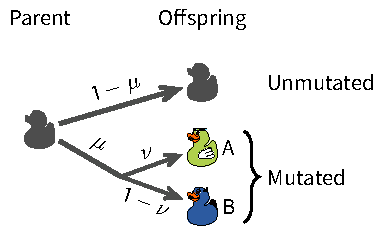
\includegraphics[width=3.5cm]{../TeXPics/mutationscheme.pdf}};
\node[right = 2cm of pic, yshift = 0.5cm, color = dgray](Y){$\mathbb{E}[Y_i]$};
\node[text width = 4cm, font = \small, below = 0cm of Y, align= center]{Expected trait of the\\offspring of individual $i$};
\node[right = 1cm of Y]{$ = (1-\mu) \, X_i + \mu \nu$.};
\end{tikzpicture}
}

\uncover<3->{
Proportion of altruists in the population:
\begin{displaymath}
\overline{X} = \frac{1}{N} \sum_{i=1}^N X_i.
\end{displaymath}
}

\uncover<4->{
\begin{center}
\begin{tikzpicture}
\node[rounded corners, fill = maincol, text opacity = 1, fill opacity = 0.5, align = center]{{\large
We want to compute 
$ \mathbb{E}[\overline{X}]$, }\\the expected proportion of altruists in the population. 
};
\end{tikzpicture}
\end{center}
}

\end{frame}



\subsubsection{Social interactions}
\begin{frame}{Social interactions}

\begin{block}{Phenotype}
\begin{displaymath}
\phi_i = \delta X_i,
\end{displaymath}
and we assume that $\delta \ll 1.$ (Selection is weak.)
\end{block}

\begin{block}<2->{Social interactions affect fecundity}
At the first order in $\delta$, 

\begin{center}
\vspace{-0.75cm}
\begin{tikzpicture}
\tikzstyle{eqt}=[inner sep = 3pt, minimum height = 1.cm, draw=none]
\node[eqt](f){$f_i$};
\node[eqt, right = 0cm of f](eq){$=$};
\node[eqt, right = 0cm of eq](one){$1$};
\node[eqt, right = 0cm of one](plus){$+$};
\node[eqt, right = 0cm of plus](delta){$\delta$};
\node[eqt, right = 0cm of delta](lp){$\Bigg($};
\node[eqt, right = 0cm of lp](b){$\bb$};
\node[eqt, right = 0cm of b](sumin){$\sum_{j \in \mathcal{D}_i\textbackslash i} \frac{X_j}{n-1}$};
\node[eqt, right = 0cm of sumin](minus){$-$};
\node[eqt, right = 0cm of minus](c){$\cc$};
\node[eqt, right = 0cm of c](self){$X_i$};
\node[eqt, right = 0cm of self](rp){$\Bigg)$};
\node[eqt, right = 0cm of rp](dot){.};

\tikzstyle{eqh}=[inner sep = 0pt, rounded corners, minimum height=1cm, opacity = 0.4]
\tikzstyle{txt}=[text width = 4.75cm, align  = center, font = \small]

\begin{pgfonlayer}{background}
\def \hpic {1.5em}
\uncover<3->{
\node[above =0cm  of b]{
\includegraphics[height = \hpic]{../Pics/gift.pdf}};
\node[eqh, fill=maincol, fit = (b)]{};

\node[eqh, fill=maincol, fit = (c)]{};
\node[above =0cm  of c]{
\includegraphics[height = \hpic]{../Pics/coins.pdf}};
}


\uncover<4->{
\node[eqh, fill = col1, fit = (sumin)]{};

\node[txt, below = 0.5cm of sumin, xshift=-0.75cm](sumint){Proportion of altruists\\among the other deme-mates};
\draw[col1] (sumin)--(sumint);
}

\uncover<5->{
\node[eqh, fill = col2, fit = (self)]{};
\node[txt, right = 0cm of sumint, text width = 4cm](selft){The cost is only paid\\by altruists};
\draw[col2](self.south)--(selft);
}
\end{pgfonlayer}
\end{tikzpicture}



\end{center}

\end{block}

\end{frame}







\section{Results}

\subsection{Calculations}


\begin{frame}{Calculations}
\begin{block}{Notation}
\begin{description}
\item[$B_i$] = $B_i(\mathbf{X}, \delta)$: expected \# of offspring of individual $i$;
\item[$D_i$] = $D_i(\mathbf{X}, \delta)$: probability that $i$ dies.
\end{description}
\end{block}
\pause
\begin{itemize}[<+->]
\item Expected proportion of altruists at $t+1$ in the proportion of altruists, conditional on the state of the population at time $t$:
%
\begin{displaymath}
\mathbb{E}[\overline{X}(t+1)|\mathbf{X}(t)] = \frac{1}{N}\sum_{i=1}^N \left[ B_i (1-\mu) X_i + (1-D_i)X_i + B_i \mu \nu \right]
\end{displaymath}

\item Take expectation and let $t\to \infty$; consider stationary distribution $\xi$
%
\begin{displaymath}
0 = \frac{1}{N} \sum_{X \in \Omega}\left[ \sum_{i=1}^N \underbrace{B_i (1-\mu) - D_i)}_{W_i} X_i + \sum_{i=1}^N B_i \mu \nu \right]\xi(\mathbf{X}, \delta, \mu)
\end{displaymath}
\end{itemize}
\end{frame}

\begin{frame}{Calculations (2)}
\vspace{-0.75\baselineskip}
\begin{itemize}
\item Selection is weak ($\delta\ll 1$) and reproductive values are all equal:
\begin{displaymath}
0 = \frac{\delta}{N} \sum_{i=1}^N \left[  \sum_{X\in\Omega}\frac{\partial W_i}{\partial \delta} X_i \xi\tikzmark{xi}(\mathbf{X}, 0, \mu) - \sum_{X \in \Omega} \mu B^*\tikzmark{lastterm} X_i \frac{\partial \xi}{\partial \delta} \right] + O(\delta^2),
\end{displaymath}
\uncover<2->{
which we rewrite as
\vspace{-0.75\baselineskip}
\begin{displaymath}
\delta \mu B^*\tikzmark{waslast} \uncover<3>{\tikz[overlay,remember picture]
   {\draw[->, maincol, thick] ($(lastterm.south)+(0,-0.25)$) to ($(waslast.north)+(0,0.5)$);}} \frac{\partial \mathbb{E}[\overline{X}]}{\partial \delta} = \frac{\delta}{N} \, \sum_{i=1}^N\mathbb{E}_0\tikzmark{E0}\left[ \frac{\partial W_i}{\partial \delta} X_i \right]  + O(\delta^2).
   \uncover<4>{\tikz[overlay,remember picture]
   {\draw[->, maincol, thick] ($(xi.south)+(0,-0.)$) to ($(E0.north)+(-0.2,0.4)$);}}
\end{displaymath}
}
\item<5-> Using partial derivatives: phenotypes
{\small
\begin{displaymath}
\frac{\partial W_i}{\partial \delta} = \sum_{k=1}^N \frac{\partial W_i}{\partial \phi_k} \frac{\partial \phi_k}{\partial \delta} = \sum_{k=1}^N \frac{\partial W_i}{\partial \phi_k} X_k.
\end{displaymath}
}
\item<6-> We obtain
\begin{displaymath}
\delta \mu B^* \frac{\partial \mathbb{E}[\overline{X}]}{\partial \delta} = \frac{\delta}{N} \, \sum_{i=1}^N \sum_{k=1}^N\frac{\partial W_i}{\partial \phi_k} \underbrace{\mathbb{E}_0\left[  X_i X_k \right]}_{P_{ik}}  + O(\delta^2).
\end{displaymath}
\end{itemize}
\end{frame}


\begin{frame}{Calculations (3)}
\begin{itemize}
\item In a subdivided population, \footnote{\citeref{Rousset \& Billiard (2000)  }}
\begin{displaymath}
\frac{\partial W_i}{\partial \phi_i} + (n-1) \frac{\partial W_i}{\partial \phi_{\textsf{in}}} + (N-n)\frac{\partial W_i}{\partial \phi_{\textsf{out}}} = 0,
\end{displaymath}
\item<2-> So
\begin{displaymath}
\hspace{-0.75cm}\delta \mu B^* \frac{\partial \mathbb{E}[\overline{X}]}{\partial \delta} = \frac{\delta}{N} \, \sum_{i=1}^N \left( \underbrace{\frac{\partial W_i}{\partial \phi_i}}_{-\mathcal{C}} + \underbrace{(n-1) \frac{\partial W_i}{\partial \phi_{\textsf{in}}}}_{\mathcal{B}} \underbrace{\frac{P_{\textsf{in}} - P_{\textsf{out}}}{P_{ii} - P_{\textsf{out}}}}_{R} \right) (P_{ii} - P_{\textsf{out}}) + O(\delta^2).
\end{displaymath}
\item<3-> Then further decompose with partial derivatives:
\begin{displaymath}
\frac{\partial W_i}{\partial \phi_k} = \sum_{\ell = 1}^N \frac{\partial W_i}{\partial f_{\ell}} \frac{\partial f_{\ell}}{\partial \phi_k}
%
\uncover<4->{\small 
\quad \textsf{and }
\frac{\partial f_{\ell}}{\partial \phi_{\ell}} = - \cc\tikzmark{c}; \quad
\frac{\partial f_{\ell}}{\partial \phi_{\textsf{in}}} = \frac{\bb\tikzmark{b}}{n-1} ; \quad
\frac{\partial f_{\ell}}{\partial \phi_{\textsf{out}}} = 0.
{\tikz[overlay,remember picture]
   {\node[above = 0cm of c] {\includegraphics[height = 1em]{../Pics/coins}};
   \node[above = 0cm of b] {\includegraphics[height = 1em]{../Pics/gift}};}}
}
\end{displaymath}
\end{itemize}
\end{frame}


\subsection{IDB}

\subsubsection{Genealogy}


\begin{frame}{Genealogy, Identity by descent and Identity in state}
\begin{center}
\begin{tikzpicture}
\def \nlines {5}
\def \ncols {10}
\def \dx {0.7cm}
\def \dy {0.9cm}
\tikzstyle{indivbase}=[circle, inner sep=0pt, text width=0.5cm, fill=bgcol, draw=none]
\tikzstyle{genlink}=[draw=fgcol, line width=1.2pt]
\foreach \i in {1,...,\nlines}{
\foreach \j in {1,...,\ncols}{
	\node[indivbase] at(\dx*\j, -\dy*\i) (c\i\j) {};
}}

\uncover<1->{
\foreach \i in {1,...,\nlines}{
\foreach \j in {1,...,\ncols}{
	\node[indivbase, draw=fgcol] at(c\i\j) {};
}}
}

\draw[->, >=angle 45] (-0.5*\dx, 0)--(-0.5*\dx, -\nlines*\dy-\dy){} node [above, anchor=north east] {Time};

\tikzstyle{iA}=[indivbase, fill=col2]
\tikzstyle{iB}=[indivbase, fill=col4]

% Genealogy
\tikzstyle{mut}=[color=col1, font=\small]
\newcommand{\symbmut}{$\bigstar$}

\uncover<2->{
\draw[genlink] (c11)--(c21);
\draw[genlink] (c11)--(c22);
\draw[genlink] (c11)--(c23);
\draw[genlink] (c13)--(c24);
\draw[genlink] (c15)--(c25);
\draw[genlink] (c17)--(c26);
\draw[genlink] (c17)--(c27);
\draw[genlink] (c17)--(c28);
\draw[genlink] (c110)--(c29);
\draw[genlink] (c110)--(c210);

\draw[genlink] (c21)--(c31);
\draw[genlink] (c21)--(c32);
\draw[genlink] (c24)--(c33);
\draw[genlink] (c25)--(c34);
\draw[genlink] (c25)--(c35);
\draw[genlink] (c26)--(c36);
\draw[genlink] (c27)--(c37);
\draw[genlink] (c28)--(c38);
\draw[genlink] (c29)--(c39);
\draw[genlink] (c29)--(c310);

\draw[genlink] (c32)--(c41);
\draw[genlink] (c32)--(c42);
\draw[genlink] (c32)--(c43);
\draw[genlink] (c35)--(c44);
\draw[genlink] (c36)--(c45);
\draw[genlink] (c36)--(c46);
\draw[genlink] (c38)--(c47);
\draw[genlink] (c38)--(c48);
\draw[genlink] (c39)--(c49);
\draw[genlink] (c310)--(c410);

\draw[genlink] (c42)--(c51);
\draw[genlink] (c42)--(c52);
\draw[genlink] (c43)--(c53);
\draw[genlink] (c45)--(c54);
\draw[genlink] (c45)--(c55);
\draw[genlink] (c46)--(c56);
\draw[genlink] (c47)--(c57);
\draw[genlink] (c47)--(c58);
\draw[genlink] (c48)--(c59);
\draw[genlink] (c48)--(c510);
}

\uncover<3->{
\node[iA] at (c11){};
\node[iA] at (c12){};
\node[iA] at (c13){};
\node[iA] at (c14){};
\node[iA] at (c15){};
\node[iA] at (c16){};
\node[iB] at (c17){};
\node[iA] at (c18){};
\node[iA] at (c19){};
\node[iA] at (c110){};
}

\uncover<4->{
\node[iA] at (c21){};
\node[iA] at (c22){};
\node[iA] at (c23){};
\node[iA] at (c24){};
\node[iA] at (c25){};
\node[iB] at (c26){};
\node[iB] at (c27){};
\node[iB] at (c28){};
\node[iA] at (c29){};
\node[iA] at (c210){};

\node[iA] at (c31){};
\node[iA] at (c32){};
\node[iA] at (c33){};
\node[iA] at (c34){};
\node[iA] at (c35){};
\node[iB] at (c36){};
\node[iB] at (c37){};
\node[iB] at (c38){};
\node[iA] at (c39){};
\node[iA] at (c310){};

\node[iA] at (c41){};
\node[iA] at (c42){};
\node[iA] at (c43){};
\node[iA] at (c44){};
\node[iB] at (c45){};
\node[iB] at (c46){};
\node[iB] at (c47){};
\node[iB] at (c48){};
\node[iA] at (c49){};
\node[iA] at (c410){};

\node[iA] at (c51){};
\node[iA] at (c52){};
\node[iA] at (c53){};
\node[iB] at (c54){};
\node[iB] at (c55){};
\node[iB] at (c56){};
\node[iB] at (c57){};
\node[iB] at (c58){};
\node[iB] at (c59){};
\node[iB] at (c510){};

}

\uncover<5->{
\path(c11)--(c21) node[midway, mut]{\symbmut};
\node[iB] at (c21){};
\node[iB] at (c31){};
\node[iB] at (c32){};
\node[iB] at (c41){};
\node[iB] at (c42){};
\node[iB] at (c43){};
\node[iB] at (c51){};
\node[iB] at (c52){};

\path(c26)--(c36) node[midway, mut]{\symbmut};
\node[iA] at (c36){};
\node[iA] at (c46){};
\node[iA] at (c45){};
\node[iA] at (c54){};
\node[iA] at (c55){};
\node[iA] at (c56){};

\path(c43)--(c53) node[midway, mut]{\symbmut};

% Mutations that did not change type
\path(c46)--(c56) node[midway, mut]{\symbmut};
\path(c17)--(c27) node[midway, mut]{\symbmut};
\path(c310)--(c410) node[midway, mut]{\symbmut};

}

\tikzstyle{pairexamples}=[rectangle, rounded corners, draw=maincol, inner sep=2pt, line width=1pt]
\uncover<6>{
\node[fit=(c53)(c54), pairexamples]{};
}
\uncover<7>{
\node[fit=(c53)(c52), pairexamples]{};
}
\uncover<8>{
\node[fit=(c56)(c55), pairexamples]{};
}
\uncover<9>{
\node[fit=(c54)(c55), pairexamples]{};
}

\end{tikzpicture}
\end{center}

\end{frame}


\subsubsection{PQ}



\begin{frame}{Expected state of pairs of sites and identity by descent}

At neutrality (i.e., in the absence of selection, $\delta = 0$),
\vspace{1em}

\begin{center}

\uncover<2->{
\begin{tikzpicture}
\tikzstyle{eqpart}=[rectangle, draw=none, inner sep=1pt, minimum height=0.55cm, rounded corners, font=\Large]
\tikzstyle{expl}=[rectangle, inner sep=2pt, draw=none, align=left, font=\small]
\tikzstyle{arrexp}=[->, >=stealth, line width=1.2pt, draw=maincol]

\def \dye {0.4cm}
\node[eqpart](Pij){$P_{ij}$};
\node[expl, below=\dye of Pij.south east, anchor=north east, align=right, text width=4.cm](eP){Expected state of the $i,j$ pair\\= Probability that the two individuals are altruists};

\draw[arrexp](Pij.south)--(eP);

\def \dx {0.25cm}
\uncover<3->{
\node[eqpart, right= \dx of Pij](equal){$=$};

\node[eqpart, right= \dx of equal](rhs1){$Q_{ij}$};
\node[eqpart, right= 0 of rhs1](rhs2){$ \nu $};
}

\uncover<3-4>{
\node[expl, anchor=north, text width=6.5cm, align=center] at ($(rhs1 |- eP.south east)+(0,-\dye)$) (e1){Probability that the individuals at sites $i$ and $j$ are identical by descent \\ (no mutation since their common ancestor)};
\draw[arrexp](rhs1)--(e1);
}

\uncover<4>{
\node[expl, anchor=west, text width=4.5cm] at ($(rhs2|-eP)+(-0.cm,0)$)(e2){Probability that a mutant is an altruist \\= Probability that a given site is occupied by an altruist};
\draw[arrexp](rhs2.south)--(e2);
}

\uncover<5->{
\node[eqpart, right= 0 of rhs2](rhs3){$ + $};
\node[eqpart, right= 0 of rhs3](rhs4){$ (1-Q_{ij})$};
\node[eqpart, right= 0 of rhs4](rhs5){$\nu^2$};
}

\uncover<5>{
\node[expl, anchor=north, text width=6cm, align=center] at ($(rhs4 |- eP.south east)+(0,-\dye)$) (e4){Probability that the individuals at sites $i$ and $j$ are not identical by descent};
\draw[arrexp](rhs4)--(e4);

\node[expl, anchor=west, text width=4.5cm] at ($(rhs5|-eP)+(-0.cm,0)$)(e5){Probability that both sites are occupied by an altruist};
\draw[arrexp](rhs5.south)--(e5);
}



\end{tikzpicture}
} % end uncover
\end{center}
\uncover<6>{
{
\Large
\begin{center}
\textcolor{col1}{$Q_{\textsf{in}}$}, \textcolor{col2}{$Q_{\textsf{out}}$}
\end{center}
}
}
\end{frame}



\subsection{EX}
\begin{frame}<1-8>[label = EXframe]{Expected frequency of altruists in the population}
\begin{center}
\begin{tikzpicture}[node distance = 0.2cm and 0.16cm, anchor = base, baseline = 0pt]
% vertical and horizontal
\tikzstyle{math}=[font=\large, inner sep = 0pt, draw = none, minimum height = 1.2cm]

\def \blsk {-1em}

\node[math, anchor = west] (EX) at(0,0){$\mathbb{E}[\overline{X}]$};
\node[math, right = of EX] (equal){$=$};
\node[math, right = of equal](nu){$\nu$};
\node[math, right = of nu](plus){$+$};
\node[math, right = of plus](sel){$\selstr$};
\node[math, right = of sel](nuvar){$\nu (1-\nu)$};
\node[math, right = of nuvar](fac){$\dfrac{1-\mu}{\mu}$};
\node[math, right = of fac](fact){$\left(1 - \Qout \right)$};
\node[math, right = of fact]{$\times$};
\node[math, below = of plus] (blocCD){$-\cc$};
\node[math, left = of blocCD]{$\Bigg($};
\node[math, right = of blocCD] (blocCI){$- \, (\bb - \cc) \left( \dfrac{(1-m)^2}{\demesize} + \dfrac{m^2}{\demesize \, (\nbdemes - 1)} \right)$};
\node[math, below = of blocCD.south west, anchor = north west](pluss){$+$};
\node[math, right = of pluss](R){$ \dfrac{\Qin - \Qout}{1 - \Qout}$};
\node[math, right = of R](lbrace){$\Bigg[$};
\node[math, right = of lbrace](blocBD){$\bb$};
\node[math, right = of blocBD](blocBI){$- \, (\bb-\cc) \, (n-1) \, \left( \dfrac{(1-m)^2}{\demesize} + \dfrac{m^2}{\demesize \, (\nbdemes - 1)} \right)$};
\node[math, right = of blocBI](rbrace){$\Bigg]$};
\node[math, right = of rbrace]{$\Bigg)$};

\tikzstyle{highlgt}=[rectangle, rounded corners = 2pt, line width = 1pt, fill opacity = 0.4, text height = 0.5cm, fill = maincol, draw = none, inner sep = 0.5pt]
\tikzstyle{explain}=[font=\normalsize, color = maincol, anchor = north west, align = left, inner sep = 1pt, font = \small]
\tikzstyle{lnk}=[draw = maincol, line width = 1.5pt]


\begin{scope}[on background layer]

\pause

\node[highlgt, fit = (nu)](hnu){};
\node[explain] at (0, 2) (enu){Mutation-drift\\equilibrium};
\path[lnk](hnu.north)--(enu);

\pause

\node[highlgt, fit = (sel)](hsel){};
\node[explain] at(2, 1.65)(esel){Selection\\strength};
\path[lnk](hsel.north)--(esel);

\pause

\node[highlgt, fit = (nuvar)](hnuvar){};
\node[explain] at(4, 2)(enuvar){Variance in the state of one site};
\path[lnk](hnuvar.north)--(enuvar);

\pause

\node[highlgt, fit = (blocCD)(blocCI), fill = col1](hC){};
\tikzstyle{explainH}=[explain, font=\LARGE, anchor = center]
\node[explainH, right = of hC, color = col1]{$-\mathcal{C} \uncover<11->{\nearrow}$};

\pause

\node[highlgt, fit =(blocBD)(blocBI), fill = col2](hB){};
\node[explainH, below = of hB, color = col2]{$\mathcal{B} \uncover<11->{\nearrow}$};

\pause

\node[highlgt, fit = (R), fill = col3](hR){};
\node[explainH, below = of hR, color = col3]{$R \uncover<9->{\searrow}$};

\uncover<12->{
\node[highlgt, fit = (fact), fill = maincol](ht){};
\node[explainH, above = of ht, color = maincol]{$\searrow$};
}

\end{scope}

\uncover<8,9>{
\tikzstyle{blind}=[rectangle, fill = bgcol, fill opacity = 0.9, inner sep = 0pt, rounded corners = 2pt]

\node[blind, fit = (blocBI)]{};
\node[blind, fit = (blocCI)]{};
}

\end{tikzpicture}
\end{center}

\uncover<9>{\phantom{{\Huge X}}}
\end{frame}



\subsubsection{R changes}
\begin{frame}{How does relatedness $R$ change with the emigration probability $m$?}

\begin{center}
\begin{tikzpicture}
\def \wpic {0.35\textwidth}

\node[](pWF){\includegraphics[width = \wpic]{../Pics/RplotWF1.pdf}};
\node[right = 2cm of pWF](pM){\includegraphics[width = \wpic]{../Pics/RplotM1.pdf}};


\node[above = 0cm of pWF]{Wright-Fisher (N deaths)};
\node[above = 0cm of pM]{Moran (1 death)};


\foreach \i in {2,5}{
\pause
{
\node[fill=white]at(pWF){\includegraphics[width = \wpic]{../Pics/RplotWF\i.pdf}};
\node[fill=white]at(pM){\includegraphics[width = \wpic]{../Pics/RplotM\i.pdf}};
}
}
\end{tikzpicture}
\btVFill 
($\demesize = 4, \nbdemes = 15$)
\end{center}
\end{frame}


\againframe<9->{EXframe}


\def \wpic {0.3\textwidth}

\begin{frame}{Effect of the emigration probability $m$ on the expected proportion of altruists}

\begin{center}
\begin{tikzpicture}
\def \wL {2cm}
\uncover<1>{
\node[](pWF){\includegraphics[width=\wpic]{{../Pics/EXWF_sel0.005_htg0_0}.pdf}};

\node[anchor=north east]at(pWF.north east) (L) {\includegraphics[width=\wL]{{../Pics/Legend_0}.pdf}};
}

\node[above = 0cm of pWF, align=center]{Wright-Fisher\\($N$ deaths \& $N$ births)};

\uncover<2>{
\node[]at(pWF) (pWFp){\includegraphics[width=\wpic]{{../Pics/EXWF_sel0.005_htg0_1}.pdf}};
\node[]at(L) {\includegraphics[width=\wL]{{../Pics/Legend_1}.pdf}};
}
\uncover<3>{
\node[]at(pWF) (pWFp){\includegraphics[width=\wpic]{{../Pics/EXWF_sel0.005_htg0_2}.pdf}};
\node[]at(L) {\includegraphics[width=\wL]{{../Pics/Legend_2}.pdf}};
}
\uncover<4>{
\node[]at(pWF) (pWFp){\includegraphics[width=\wpic]{{../Pics/EXWF_sel0.005_htg0_3}.pdf}};
\node[]at(L) {\includegraphics[width=\wL]{{../Pics/Legend_3}.pdf}};
}
\uncover<5->{
\node[]at(pWF) (pWFp){\includegraphics[width=\wpic]{{../Pics/EXWF_sel0.005_htg0_4}.pdf}};
\node[]at(L) {\includegraphics[width=\wL]{{../Pics/Legend_4}.pdf}};
}

\uncover<6>{
\node[right = 1ex of pWF](pM){\includegraphics[width=\wpic]{{../Pics/EXBD_sel0.005_htg0_0}.pdf}};
}
\uncover<6->{
\node[above = 0cm of pM, align = center]{Moran Birth-Death\\ ($1$ birth \& $1$ death)};
}
\uncover<7>{
\node[]at(pM) (pMp){\includegraphics[width=\wpic]{{../Pics/EXBD_sel0.005_htg0_1}.pdf}};
}
\uncover<8->{
\node[]at(pM) (pMp){\includegraphics[width=\wpic]{{../Pics/EXBD_sel0.005_htg0_4}.pdf}};
}

\uncover<9>{
\node[right = 1ex of pM](pDB){\includegraphics[width=\wpic]{{../Pics/EXDB_sel0.005_htg0_0}.pdf}};
}
\uncover<9->{
\node[above = 0cm of pDB, align = center]{Moran Death-Birth\\ ($1$ death \& $1$ birth)};
}

\uncover<10>{
\node[]at(pDB) (pDBp){\includegraphics[width=\wpic]{{../Pics/EXDB_sel0.005_htg0_1}.pdf}};
}

\uncover<11>{
\node[]at(pDB) (pDBp){\includegraphics[width=\wpic]{{../Pics/EXDB_sel0.005_htg0_2}.pdf}};
}

\uncover<12>{
\node[]at(pDB) (pDBp){\includegraphics[width=\wpic]{{../Pics/EXDB_sel0.005_htg0_3}.pdf}};
}
\uncover<13>{
\node[]at(pDB) (pDBp){\includegraphics[width=\wpic]{{../Pics/EXDB_sel0.005_htg0_4}.pdf}};
}
\end{tikzpicture}

\btVFill
{\small ($b=15, c=1, \demesize = 4, \nbdemes = 15, \selstr = 0.005$)}
\end{center}

\end{frame}


\subsection{Explanation}

\begin{frame}{How to explain this result? (Moran Death-Birth)}

\vspace{-0.5cm}

\begin{displaymath}
{\color{col1}-\mathcal{C}} + \color{col2}{\mathcal{B}} \color{col3}{R} \color{fgcol}> 0 \Leftrightarrow {\color{col3}R} > {\color{col1}\mathcal{C}}/{\color{col2}\mathcal{B}}
\end{displaymath}

\vspace{-0.75cm}

\uncover<2->{
\begin{center}
\alt<3->{\includegraphics[height=0.7\textheight]{../../Programs/R/Pics/explainDB.pdf}}{\includegraphics[height=0.7\textheight]{../Pics/explainDB_justR.pdf}}
\end{center}
}
\end{frame}

\subsection{Robustness}

\begin{frame}

\begin{center}
{\LARGE \color{maincol} Is the result robust?}
\end{center}
\end{frame}

\def \wpic {0.3\textwidth}
\begin{frame}{Strong selection}
\begin{center}

\begin{tikzpicture}

\uncover<1>{
\node[] (pWFs){\includegraphics[width=\wpic]{{../Pics/EXWF_sel0.005_htg0_4}.pdf}
};
\node[above= 0cm of pWFs, align=center]{Wright-Fisher,\\ weak selection};


\node[right = 0cm of pWFs](pBDs){\includegraphics[width=\wpic]{{../Pics/EXBD_sel0.005_htg0_4}.pdf}
};
\node[above= 0cm of pBDs, align=center]{Moran Death-Birth,\\ weak selection};

\node[right = 0cm of pBDs](pDBs){\includegraphics[width=\wpic]{{../Pics/EXDB_sel0.005_htg0_4}.pdf}
};
\node[above= 0cm of pDBs, align=center]{Moran Death-Birth,\\ weak selection};
}

\uncover<2>{
\node[] (pWFs){\includegraphics[width=\wpic]{{../Pics/EXWF_sel0.1_htg0}.pdf}
};
\node[above= 0cm of pWFs, align=center]{Wright-Fisher,\\ strong selection};


\node[right = 0cm of pWFs](pBDs){\includegraphics[width=\wpic]{{../Pics/EXBD_sel0.1_htg0}.pdf}
};
\node[above= 0cm of pBDs, align=center]{Moran Death-Birth,\\ strong selection};

\node[right = 0cm of pBDs](pDBs){\includegraphics[width=\wpic]{{../Pics/EXDB_sel0.1_htg0}.pdf}
};
\node[above= 0cm of pDBs, align=center]{Moran Death-Birth,\\ strong selection};
}


\end{tikzpicture}
\alt<2>{\btVFill
{\small ($b=15, c=1, \demesize = 4, \nbdemes = 15, \selstr = 0.1$)}
}{\btVFill
{\small ($b=15, c=1, \demesize = 4, \nbdemes = 15, \selstr = 0.005$)}
}
\end{center}
\end{frame}




\begin{frame}{Heterogeneous deme sizes ($\overline{n} = 4$ as before, but $2\leq n \leq 5$)}
\begin{center}
\begin{tikzpicture}
\node[] (pWFs){\includegraphics[width=\wpic]{{../Pics/EXWF_sel0.005_htg1}.pdf}
};
\node[above= 0cm of pWFs, align=center]{Wright-Fisher\\};


\node[right = 0cm of pWFs](pBDs){\includegraphics[width=\wpic]{{../Pics/EXBD_sel0.005_htg1}.pdf}
};
\node[above= 0cm of pBDs, align=center]{Moran Death-Birth\\ };

\node[right = 0cm of pBDs](pDBs){\includegraphics[width=\wpic]{{../Pics/EXDB_sel0.005_htg1}.pdf}
};
\node[above= 0cm of pDBs, align=center]{Moran Death-Birth\\ };
\end{tikzpicture}
\btVFill
{\small ($b=15, c=1, \overline{\demesize} = 4, \nbdemes = 15, \selstr = 0.005$)}

\end{center}
\end{frame}


\begin{frame}{Political implications}
\only<1>{
\begin{center}
\includegraphics[width=0.55\textwidth]{../Pics/rBCcake.pdf}
\end{center}
}
\vspace{-\baselineskip}
\only<2->{
\begin{center}
\begin{tikzpicture}
\node[anchor=center]at(0,0)(abs){\includegraphics[width=0.75\textwidth]{../Pics/Kummerli1.pdf}
};
\tikzstyle{exc}=[draw, inner sep = 0pt, drop shadow, line width=1.5pt]

\uncover<3->{
\node[exc]at(-1,0.85){\includegraphics[width=0.6\textwidth]{../Pics/Kummerli2.pdf}};

\node[exc]at(1,-2){\includegraphics[width=0.6\textwidth]{../Pics/Kummerli3.pdf}};
}
\end{tikzpicture}
\end{center}
}
\end{frame}




\section{THM}


\begin{frame}{Take-Home Messages}


\begin{center}
\begin{minipage}{0.9\textwidth}

\begin{itemize}
\item<+-> Under weak selection, it is
possible to compute the expected frequency of social
individuals, for any life-cycle, any regular population structure,  any mutation probability. \hspace{\stretch{1}}{\footnotesize \textcolor{mgray}{(D., 2017, JTB)}}

\item<+-> $\mathbb{E}[\overline{X}]>\nu \Leftrightarrow \mathcal{B}\, R > \mathcal{C}$.

\item<+-> In subdivided populations, $\mathbb{E}[\overline{X}]$ can increase with the emigration probability $m$ when strategy transmission is imperfect ($\mu > 0$).  \hspace{\stretch{1}}{\footnotesize \textcolor{mgray}{(D., \textit{in review.})}}


\item<+-> This result seems to hold under stronger selection \\and in heterogeneous populations.
\end{itemize}
\end{minipage}
\end{center}


\uncover<+->{


\btVFill
\hrule
\begin{block}{Funding \& Thanks}
\begin{center}
\vspace{-0.25cm}

\begin{tikzpicture}
\node[](anr){\includegraphics[height = 1cm]{/home/florencedebarre/Dropbox/Presentations/GlobalPics/logo_anr.pdf}};
\node[below = 0cm of anr, font = \small](anrn){ANR-14-ACHN-0003-01};

\node[right = of anrn.south east, align = center, anchor = south west](Ch){A. Lambert \\ {\small for organizing the workshop}};

\node[right = of Ch, color = maincol, text width = 4cm, font = \large, align = center]{and thank you for your attention!};

\end{tikzpicture}
\end{center}

\end{block}
}
\end{frame}

\end{document}



\subsection{Population structure}

\begin{frame}{Subdivided population -- Island model}

$\nbdemes$ demes \uncover<2->{of $\demesize$ individuals each (total population size $N = \demesize \,\nbdemes$)}
\begin{center}

\begin{tikzpicture}
\tikzstyle{bigpop}=[circle, line width = 0.7pt, draw = none, fill = maincol!40, minimum width = 2.75cm]

\node[bigpop]at(0,0)(p4){};
\node[bigpop]at(2.5,2)(p3){};
\node[bigpop]at(2.5,-2)(p2){};
\node[bigpop]at(5,0)(p1){};
\node[bigpop]at(7.5,2)(p5){};
\node[bigpop]at(7.5,-2)(p6){};
\node[bigpop]at(10,0)(p7){};

\uncover<2->{
\def \wsmall {0.7cm}
\tikzstyle{site}=[circle, line width = 1.5pt, draw = maincol, fill=bgcol, minimum width = \wsmall]

\def \rad {0.85cm}
\foreach \i in {1,...,7}{
\foreach \j in {1,...,3}{
\node[site] at ($(p\i) + (90+\j * 120:\rad)$) (p\i\j){};
}
\node[site] at (p\i) (p\i4){};
}

% Philopatry
\uncover<3->{
\path (p1) edge [loop above, ->, looseness = 5, line width = 4pt, font = \large] node [above]{$1-m$} (p1);
}

% Dispersal
\uncover<4->{
\foreach \i in {2,...,7}{
\path[line width =1.5pt, ->, draw](p1)--(p\i);
}
\node[align = center, below = 0cm of p1, text width = 3cm, font = \large]{$m$\\Emigration probability};
}

\uncover<5->{
\tikzstyle{focusing}=[circle, minimum width = \wsmall, fill opacity = 0.8]
\node[focusing, fill = mgray] at (p14){};

\node[anchor = north , draw, align = center, font = {\bf\large}]at(10, -1.75){\color{mgray}focal \\ {\uncover<6->{\color{col1} in}} \\ {\uncover<7->{ \color{col2} out}}};

}

\uncover<6->{
\foreach \i in {1,...,3}{
\node[focusing, fill = col1] at (p1\i){};
}
}

\uncover<7->{
\foreach \i in {2,...,7}{
\foreach \j in {1,...,4}{
\node[focusing, fill = col2] at (p\i\j){};
}}
}



% Add ducks
\foreach \i in {1,...,7}{
\foreach \j in {1,...,4}{
\node[]at(p\i\j) {\includegraphics[height = 0.6cm]{../Pics/type0.pdf}};
}}

% Add presents
\uncover<8->{
\foreach \i in {1,...,7}{
\foreach \j in {1,...,3}{
\node[]at($(p\i) + (30+ 120*\j:0.75cm)$){\includegraphics[height = 0.5cm]{../Pics/gift.pdf}};
}}
}


}
\end{tikzpicture}
\end{center}

\end{frame}

\subsection{Updating the population}

\begin{frame}{Updating the population}
\begin{center}

\begin{columns}
\begin{column}{0.5\textwidth} 
Constant population size ($N$), so\\
between two time steps, 

\newcommand{\Ddead}{\includegraphics[height=0.75cm]{../Pics/death}}
\newcommand{\Dbaby}{\includegraphics[height=0.75cm]{../Pics/birth}}
{\Large 
\begin{tikzpicture}
\def \ndim {-0.25cm}
\tikzstyle{textrec}=[rectangle, minimum width=2cm]
\node[textrec] at (0,0) (Ge){$=$};
\node[textrec, left of = Ge] (G1){$\# \vcenter{\hbox{\Ddead}}$};
\node[textrec, right of =Ge] (G2){$\# \vcenter{\hbox{\Dbaby}}$};

\uncover<2->{
\node[textrec]at (0,-2) (Ae){$=$};
\node[textrec, left of = Ae] (A1){$N \, \vcenter{\hbox{\Ddead}}$};
\node[textrec, right of =Ae] (A2){$N \, \vcenter{\hbox{\Dbaby}}$};

\node[below =\ndim of A1]{$\vdots$};
\node[below =\ndim of A2]{$\vdots$};
\node[below =\ndim of Ae](de){};

\node[textrec, below of = de, anchor=north] (Be){$=$};
\node[textrec, left of = Be] (B1){$k \, \vcenter{\hbox{\Ddead}}$};
\node[textrec, right of =Be] (B2){$k \, \vcenter{\hbox{\Dbaby}}$};

\node[below =\ndim of B1]{$\vdots$};
\node[below =\ndim of B2]{$\vdots$};
\node[below =\ndim of Be](de2){};

\node[textrec, below of = de2, anchor=north] (Ce){$=$};
\node[textrec, left of = Ce] (C1){$1 \, \vcenter{\hbox{\Ddead}}$};
\node[textrec, right of =Ce] (C2){$1 \, \vcenter{\hbox{\Dbaby}}$};

\path[->, draw, >=latex, line width=1pt] (C1.west)--(A1.west);
}

\uncover<3->{
\node[textrec, right = 0cm of A2.east, font=\normalsize]{Wright-Fisher};

\node[textrec, right = 0cm of C2.east, align=center, font=\normalsize]{Moran process};

}
\end{tikzpicture}
}

\end{column}

\begin{column}{0.47\textwidth} 
\begin{center}
\uncover<4->{
\textcolor{maincol}{Life-cycle}\\
\uncover<8->{``Death-Birth'' updating}
}

\vspace{1em}
\begin{tikzpicture}
\def \xx {2.25}

\tikzstyle{lcstep}=[rectangle, rounded corners, text width=3cm, minimum height=1.25cm, align=center, fill=bgcol!20, inner sep=2pt, font=\normalsize]

\tikzstyle{lcpath}=[->, draw, bend left=30, line width=1.2pt]

\uncover<5->{
\draw[lcpath] (90:\xx) arc (90:90-90+22:\xx){};
}
\uncover<6->{
\draw[lcpath] (0:\xx) arc (0:0-90+45:\xx){};
}
\uncover<7->{
\draw[lcpath] (180:\xx) arc (180:180-90+45:\xx){};
\draw[lcpath] (270:\xx) arc (270:270-90+22:\xx){};
}

\uncover<4->{
\node[lcstep](lc1) at (0,\xx){Offspring\\ production};
}

\uncover<5->{
\node[lcstep](lc2) at (\xx,0){Offspring\\ dispersal};
}
\uncover<6->{
\node[lcstep](lc3) at (0, -\xx){$k$ parents die};
}
\uncover<7->{
\node[lcstep](lc4) at (-\xx, 0){Establishment of\\ $k$ offspring};
}
\end{tikzpicture}

\end{center}

\end{column}
\end{columns}


\end{center}

\end{frame}
